%%%%%%%%%%%%%%%%%%%%%%%%%%%%%%%%%%%%%%%%%%%%%%%%%%%%%%%%%%%%%%%%%%%%%%%%%%%%%%%%%%%%%%%%%%%%%%
%
%                                                       Example IS Template
%
% \documentclass{woosterthesis} must be at the beginning of every IS. Options are the same as
% for the report class with some additional options, abstractonly, blacklinks, code, kaukecopyright, palatino, picins,
% maple, index, verbatim, dropcaps, euler, gauss, alltt,  woolshort, colophon, woosterchicago, and
% achemso. The kaukecopyright option will put the arch symbol with the word mark on the
% copyright page. The woosterthesis class is based on the report class. One thing to note is that
% the ``%'' symbol comments out all characters that follow it on the line.
%%%%%%%%%%%%%%%%%%%%%%%%%%%%%%%%%%%%%%%%%%%%%%%%%%%%%%%%%%%%%%%%%%%%%%%%%%%%%%%%%%%%%%%%%%%%%%

%%%%%%%%%%%%%%%%%%%%%%%%%%%%%%%%%%%%%%%%%%%%%%%%%%%%%%%%%%%%%%%%%%%%%%%%%%%%%%%%%%%%%%%%%%%%%%
% use this declaration for a draft  version of your IS
\documentclass[10pt,palatino,code,picins,kaukecopyright,openright,woolshort,dropcaps,verbatim,index,euler]{woosterthesis}
%\documentclass[10pt,code,picins,kaukecopyright,openright,woolshort,dropcaps,verbatim,euler,index,colophon,blacklinks,twoside]{woosterthesis}
% note that you can specify the woosterchicago option to use Chicago citation style and achemso to use the American Chemical Society citation format
%
%%%%%%%%%%%%%%%%%%%%%%%%%%%%%%%%%%%%%%%%%%%%%%%%%%%%%%%%%%%%%%%%%%%%%%%%%%%%%%%%%%%%%%%%%%%%%%
% use this declaration for the print version of your IS
%\documentclass[12pt,code,palatino,picins,blacklinks,kaukecopyright,openright,twoside]{woosterthesis} % probably what most students would use
%
%%%%%%%%%%%%%%%%%%%%%%%%%%%%%%%%%%%%%%%%%%%%%%%%%%%%%%%%%%%%%%%%%%%%%%%%%%%%%%%%%%%%%%%%%%%%%%
% use this declaration for the CD version of your IS
%\documentclass[12pt,code,palatino,picins,kaukecopyright,openright,twoside]{woosterthesis}
%%%%%%%%%%%%%%%%%%%%%%%%%%%%%%%%%%%%%%%%%%%%%%%%%%%%%%%%%%%%%%%%%%%%%%%%%%%%%%%%%%%%%%%%%%%%%%

%%%%%%%%%%%%%%%%%%%%%%%%%%%%%%%%%%%%%%%%%%%%%%%%%%%%%%%%%%%%%%%%%%%%%%%%%%%%%%%%%%%%%%%%%%%%%%
%
%                                                       Load Packages
%
%   To load packages in addition to the ones that are loaded by default, please place your
%   usepackage commands in the packages.tex file in the styles folder.
%
%
%%%%%%%%%%%%%%%%%%%%%%%%%%%%%%%%%%%%%%%%%%%%%%%%%%%%%%%%%%%%%%%%%%%%%%%%%%%%%%%%%%%%%%%%%%%%%%

%%%%%%%%%%%%%%%%%%%%%%%%%%%%%%%%%%%%%%%%%%%%%%%%%%%%%%%%%%%%%%%%%%%%%%%%%%%%%%%%%%%%%%%%%%%%%%
%
%                                                       Packages
%
% Do not add any other packages without consulting with Dr. Breitenbucher as they may break the functionality of the class.
%
%%%%%%%%%%%%%%%%%%%%%%%%%%%%%%%%%%%%%%%%%%%%%%%%%%%%%%%%%%%%%%%%%%%%%%%%%%%%%%%%%%%%%%%%%%%%%%

\ifxetex%
	\defaultfontfeatures{Mapping=tex-text}%
		\setmainfont[Numbers=OldStyle,BoldFont={* Semibold}]{Adobe Garamond Pro}% select the body font other choices would be Baskerville, Optima Regular, Didot, Georgia, Cochin
                      \setmathrm{Adobe Garamond Pro}
                      \setmathfont[Digits,Latin]{Adobe Garamond Pro}
		\setsansfont[Scale=.87,Fractions=On,Numbers=Lining]{Myriad Pro}% select the sans serif font other choices would be Skia, Arial, Helvetica, Helvetica Neue
%		\setmonofont[Scale=.88,Fractions=On]{Prestige Elite Std Bold}% set the mono font other choices would be Courier, Monaco, American Typewriter
	           \setmonofont[Scale=.9]{Courier Std}%
%	    \setromanfont[Fractions=On,Numbers=OldStyle, BoldFont={Warnock Pro Semibold}]{Warnock Pro}%
%	    \setsansfont[Scale=.95,Fractions=On,Numbers=Lining]{Myriad Pro}%
%	    \setmonofont[Scale=.91,Fractions=On]{Courier Std Medium}%
%	    \setmonofont[Scale=.88,Fractions=On]{American Typewriter}%
%		\setmonofont[Scale=.94,Fractions=On]{Prestige Elite Std Bold}
%    		\setromanfont[Fractions=On,Numbers=OldStyle]{Minion Pro}
 %    	\setsansfont[Scale=.9,Fractions=On,Numbers=Lining]{Myriad Pro}
%     	\setmonofont[Scale=.93,Fractions=On]{Courier Std Medium}
%     	\setromanfont[Fractions=On,Numbers=OldStyle]{Minion Pro}
%     	\setsansfont[Scale=.85,Fractions=On,Numbers=Lining]{News Gothic Std}
%    		\setmonofont[Scale=.93,Fractions=On]{Prestige Elite Std}
%		\setromanfont[Fractions=On,Numbers=OldStyle]{Minion Pro}
%		\setsansfont[Scale=.9,Fractions=On,Numbers=Lining]{Bell Gothic Std Bold}
%		\setmonofont[Scale=.95,Fractions=On]{Prestige Elite Std Bold}
\fi

%%%%%%%%%%%%%%%%%%%%%%%%%%%%%%%%%%%%%%%%%%%%%%%%%%%%%%%%%%%%%%%%%%%%%%%%%%%%%%%%%%%%%%%%%%%%%%
%
%                                                       Load Personal commands
%                                                                    
% There will be certain commands that you use frequently in the thesis. You can give these
% commands new names which are easier for you to remember. You can also combine several
% commands into a new command of your own. See The LaTeX Companion or Guide to LaTeX
% for examples on defining your own commands. These are commands that I defined to cut
% down on typing. You can enter your commands in the personal.tex file in the styles folder.
%
%%%%%%%%%%%%%%%%%%%%%%%%%%%%%%%%%%%%%%%%%%%%%%%%%%%%%%%%%%%%%%%%%%%%%%%%%%%%%%%%%%%%%%%%%%%%%%

%%%%%%%%%%%%%%%%%%%%%%%%%%%%%%%%%%%%%%%%%%%%%%%%%%%%%%%%%%%%%%%%%%%%%%%%%%%%%%%%%%%%%%%%%%%%%%
%
%                                                       Personal Commands
%                                                                    
% There will be certain commands that you use frequently in the thesis. You can give these
% commands new names which are easier for you to remember. You can also combine several
% commands into a new command of your own. See The LaTeX Companion or Guide to LaTeX for
% examples on defining your own commands. These are commands that I defined to cut down on typing.
%
%%%%%%%%%%%%%%%%%%%%%%%%%%%%%%%%%%%%%%%%%%%%%%%%%%%%%%%%%%%%%%%%%%%%%%%%%%%%%%%%%%%%%%%%%%%%%%

\newcommand{\fl}{\ell}
\newcommand{\lt}{\LaTeX\ }
\newcommand{\msw}{Word\texttrademark\ }
\newcommand{\xt}{\ifthenelse{\boolean{xetex}}{\XeTeX\ }{XeTeX} }
%\newcommand{\Cl}{\ensuremath{\textup{C}_\fl}}
%\newcommand{\bCl}{C$_{\ell}$}
%\newcommand{\Al}{\ensuremath{\textup{A}_\fl}}
%\newcommand{\msum}{{(m_1+\cdots+m_\ell)}}
%\newcommand{\Nsum}{{(N_1+\cdots+N_\ell)}}
%\newcommand{\ysum}{{(y_1+\cdots+y_\ell)}}
%\newcommand{\Nsub}{{N_1+\cdots+N_\ell}}
%\newcommand{\ysub}{{y_1+\cdots+y_\ell}}
%\newcommand{\xsub}{{x_1+\cdots+x_\ell}}
%\newcommand{\ysqsum}{{y_1^2+\cdots +y_{\fl}^2}}
%\newcommand{\msqsum}{{m_1^2+\cdots +m_{\fl}^2}}
%\newcommand{\ratio}{\left(\frac{\beta}{\alpha}\right)}
%\newcommand{\LT}{\ensuremath{\LaTeX{}}}

%%%%%%%%%%%%%%%%%%%%%%%%%%%%%%%%%%%%%%%%%%%%%%%%%%%%%%%%%%%%%%%%%%%%%%%%%%%%%%%%%%%%%%%%%%%%%%
% These commands have one argument and are entered as \commandname{argument}.
%%%%%%%%%%%%%%%%%%%%%%%%%%%%%%%%%%%%%%%%%%%%%%%%%%%%%%%%%%%%%%%%%%%%%%%%%%%%%%%%%%%%%%%%%%%%%%

%\newcommand{\bd}[1]{\textbf{#1}}
\newcommand{\mbd}[1]{{\mathbf{#1}}}
%\newcommand{\abs}[1]{\vert{#1}\vert}
\newcommand{\bvec}[1]{{\mbd{#1}}}
%\newcommand{\lvec}[1]{\abs{\bvec{#1}}}
%\newcommand{\nesmallprod}[1]{\prod_{\substack{#1=1\\
%#1\neq p}}^{\fl}}
%\newcommand{\esec}[1]{e_{2}({#1}_1,\ldots ,{#1}_\fl)}
%\newcommand{\smallprod}[1]{\prod_{#1=1}^{\fl}}
%\newcommand{\incsum}[1]{{#1}_2+2{#1}_3+\cdots +(\fl -1){#1}_\fl}
%\newcommand{\binomsum}[1]{\binom{{#1}_1}{2}+\cdots +\binom{{#1}_\fl}{2}}
%\newcommand{\imultsum}[1]{\multsum{{#1}_k\ge 0}{k=1,\ldots ,\fl}}
%\newcommand{\diagsum}[1]{\sum _{\substack{{#1}_k\ge 0\\
%k=1, \ldots ,\fl\\
%\lvec{#1}=m}}}
%\newcommand{\Mb}[1][\fl]{\ensuremath{\textup{\bd{M}}_b^{(#1)}}}
%\newcommand{\HLV}[1]{\ensuremath{\textup{\bd{H}}_{#1}}}
%\newcommand{\Rq}[1][p]{\ensuremath{\textup{R}_q^{(#1)}}}
\newcommand{\degree}[1]{\ensuremath{#1^{\circ}}}
\newcommand{\ip}[1]{\texttt{#1}\index{packages!#1}}
\newcommand{\ic}[1]{\texttt{$\backslash$#1}\index{commands!#1}}
\newcommand{\ie}[1]{#1\index{#1}}

%%%%%%%%%%%%%%%%%%%%%%%%%%%%%%%%%%%%%%%%%%%%%%%%%%%%%%%%%%%%%%%%%%%%%%%%%%%%%%%%%%%%%%%%%%%%%%
% These commands have 2 or more arguments some with default values for the first argument. You
% can learn a lot about constructing complicated equations by studying the commands in this %section.
%%%%%%%%%%%%%%%%%%%%%%%%%%%%%%%%%%%%%%%%%%%%%%%%%%%%%%%%%%%%%%%%%%%%%%%%%%%%%%%%%%%%%%%%%%%%%%

%\newcommand{\qbinom}[2]{\ensuremath{\left[{#1}\atop{#2}\right]_q}}
%\newcommand{\sqprod}[2]{\prod_{#1,#2=1}^{\fl}}
%\newcommand{\triprod}[2]{\prod_{1\le #1<#2\le \fl}}
%\newcommand{\nesqprod}[2]{\prod_{\substack{#1,#2=1\\
%#1,#2\neq p}}^{\fl}}
%\newcommand{\netriprod}[2]{\prod_{\substack{1\le #1<#2\le \fl\\
%#1,#2\neq p}}}
\newcommand{\qrfac}[3][\ ]{\left({#2}\right)_{#3}^{#1}}
%\newcommand{\multsum}[2]{\sum_{\substack{{#1}\\
%\\
%{#2}}}}
%\newcommand{\fmultsum}[2][N]{\multsum{0\le {{#2}_k}\le {{#1}_k}}{k=1,\ldots ,\fl}}
%\newcommand{\pq}[2]{\ _{#1}\varphi_{#2}}
%\newcommand{\mess}[2][y_k]{\frac{\qrfac{\alpha x_k}{#2}\qrfac{qx_k\beta^{-1}}{#2}}{\qrfac{\beta x_k}{#1}
%\qrfac{qx_k\alpha^{-1}}{#1}}}
%\newcommand{\MG}[7][\fl]{\ensuremath{\left[\textup{MG}\right]_{#2}^{(#1)}{#3}q;{#4};{#5}^{#6}{#7}}}

%%%%%%%%%%%%%%%%%%%%%%%%%%%%%%%%%%%%%%%%%%%%%%%%%%%%%%%%%%%%%%%%%%%%%%%%%%%%%%%%%%%%%%%%%%%%%%
% These commands define new environments
%%%%%%%%%%%%%%%%%%%%%%%%%%%%%%%%%%%%%%%%%%%%%%%%%%%%%%%%%%%%%%%%%%%%%%%%%%%%%%%%%%%%%%%%%%%%%%

\newcounter{unnumft}
\setcounter{unnumft}{0}
\newenvironment{unnumft}[2]{\renewcommand{\thefootnote}{}\footnote{#1}\footnote{#2}} {\addtocounter{footnote}{-2}}
\newenvironment{wooexample}{\small
\begin{singlespace}
\begin{example}}{\end{example}
\end{singlespace}}

\graphicspath{{./figures/}}% for setting where to look for figures
\citestyle{wooster}% change the style of citations. Math and CS people should leave this alone.






%%%%%%%%%%%%%%%%%%%%%%%%%%%%%%%%%%%%%%%%%%%%%%%%%%%%%%%%%%%%%%%%%%%%%%%%%%%%%%%%%%%%%%%%%%%%%%
%
%                                                       Load Theorem formatting information
%
%  If you need to define an new theorem style or want to see what theorem like environments 
%  are available please look at the theorems.tex file in the styles folder.
%
%%%%%%%%%%%%%%%%%%%%%%%%%%%%%%%%%%%%%%%%%%%%%%%%%%%%%%%%%%%%%%%%%%%%%%%%%%%%%%%%%%%%%%%%%%%%%%

%%%%%%%%%%%%%%%%%%%%%%%%%%%%%%%%%%%%%%%%%%%%%%%%%%%%%%%%%%%%%%%%%%%%%%%%%%%%%%%%%%%%%%%%%%%%%%
%
% This is where one would tell \LaTeX{} how to format Theorems, Definitions, etc. and also
% indicate the environment names. You need the amsthm package (loaded in the woosterthesis %class) in order for these commands to work.
%
%%%%%%%%%%%%%%%%%%%%%%%%%%%%%%%%%%%%%%%%%%%%%%%%%%%%%%%%%%%%%%%%%%%%%%%%%%%%%%%%%%%%%%%%%%%%%%

% an example of defining your own theoremstyle
%\newtheoremstyle{break}% name
%  {\topsep}%      Space above
%  {\topsep}%      Space below
%  {\itshape}%         Body font
%  {}%         Indent amount (empty = no indent, \parindent = para indent)
%  {\bfseries}% Thm head font
%  {.}%        Punctuation after thm head
%  {\newline}%     Space after thm head: " " = normal interword space;
%        %       \newline = linebreak
%  {}%         Thm head spec (can be left empty, meaning `normal')
\newtheoremstyle{scthm}{\topsep}{\topsep}{\itshape}{}{\bfseries\scshape}{}{ }{}% small cap font for the heading
\newtheoremstyle{itdefn}{\topsep}{\topsep}{\itshape}{}{\bfseries}{.}{ }{}% italic definitions
\newtheoremstyle{scdefn}{\topsep}{\topsep}{\itshape}{}{}{}{ }{\thmname{\textbf{#1}}\thmnumber{ \textbf{#2}}\thmnote{ \scshape #3:}}% small cap headings and italic text.

\theoremstyle{break}% this theoremstyle will put the text of the theorem on a new line.
\newtheorem{thm}{Theorem}[chapter]%number theorems within chapters 
%\newtheorem{cor}[thm]{Corollary}%by using [thm] we are numbering these environments with the theorems.
\newtheorem{cor}{Corollary}[chapter]%number corollaries within chapters .
%\newtheorem{lem}[thm]{Lemma}
\newtheorem{lem}{Lemma}[chapter]
%\newtheorem{prop}[thm]{Proposition}
\newtheorem{prop}{Proposition}[chapter]

\theoremstyle{scdefn}
%\newtheorem{defn}[thm]{Definition}
\newtheorem{defn}{Definition}[chapter]
\theoremstyle{remark}
%\newtheorem{rem}[thm]{Remark}
\newtheorem{rem}{Remark}[chapter]
\renewcommand{\therem}{}
%\newtheorem{ex}[thm]{Example}
\newtheorem{ex}{Example}[chapter]

\theoremstyle{plain}
%\newtheorem{note}[thm]{Notation}
\newtheorem{note}{Notation}[chapter]
\renewcommand{\thenote}{}
%\newtheorem{nts}[thm]{Note to self}%use to remind yourself of things yet to do
\newtheorem{nts}{Note to self}[chapter]
\renewcommand{\thents}{}
%\newtheorem{terminology}[thm]{Terminology}
\newtheorem{terminology}{Terminology}[chapter]
\renewcommand{\theterminology}{}

\theoremstyle{itdefn}
\newtheorem{bdefn}{Definition}[chapter]
\newsavebox{\fmbox} 
\newenvironment{boxeddefn}[2] 
{\begin{lrbox}{\fmbox}\begin{minipage}{0.9 \linewidth }\begin{singlespace}\begin{bdefn}[{#1}]\label{#2}\vspace{0.2cm}} 
{\end{bdefn}\end{singlespace}\end{minipage}\end{lrbox}\fbox{\usebox{\fmbox}}}

\setcounter{secnumdepth}{5}% controls the numbering of sections
\setcounter{tocdepth}{6}% controls the number of levels in the Contents

%%%%%%%%%%%%%%%%%%%%%%%%%%%%%%%%%%%%%%%%%%%%%%%%%%%%%%%%%%%%%%%%%%%%%%%%%%%%%%%%%%%%%%%%%%%%%%
% This is where one enters the information about the thesis.
%%%%%%%%%%%%%%%%%%%%%%%%%%%%%%%%%%%%%%%%%%%%%%%%%%%%%%%%%%%%%%%%%%%%%%%%%%%%%%%%%%%%%%%%%%%%%%


\title{Almost Real: An investigation into the metaphysics of virtual reality.}
\thesistype{Example Independent Study Thesis} % you should make this Independent Study Thesis
\author{Zachary A Phillips-Gary}
%\presentdegrees{Ph.D.} % you should comment this line
\degreetoobtain{Bachelor of Arts In Computer Science and Philosophy}
\presentschool{The College of Wooster}
\academicprogram{Department of Math and Computer Science }
\gradyear{2016}
\advisor{Denise Byres, Ph.D}
\secondadvisor{Elizabeth Schiltz, Ph.D}
%\reader{Reader}
\copyrighted   
%\copyrightdate{}                  
\makeindex % comment this line if you do not have an index

%%%%%%%%%%%%%%%%%%%%%%%%%%%%%%%%%%%%%%%%%%%%%%%%%%%%%%%%%%%%%%%%%%%%%%%%%%%%%%%%%%%%%%%%%%%%%%
% This is where the commands for the document begin. All \LaTeX{} documents must have a
% \begin{document} text .... \end{document} structure.
%%%%%%%%%%%%%%%%%%%%%%%%%%%%%%%%%%%%%%%%%%%%%%%%%%%%%%%%%%%%%%%%%%%%%%%%%%%%%%%%%%%%%%%%%%%%%%

\begin{document}

%%%%%%%%%%%%%%%%%%%%%%%%%%%%%%%%%%%%%%%%%%%%%%%%%%%%%%%%%%%%%%%%%%%%%%%%%%%%%%%%%%%%%%%%%%%%%%
% The front matter includes acknowledgments, dedications, vitas, list of tables, list of figures,
% copyright, abstract, title page, and contents.
%%%%%%%%%%%%%%%%%%%%%%%%%%%%%%%%%%%%%%%%%%%%%%%%%%%%%%%%%%%%%%%%%%%%%%%%%%%%%%%%%%%%%%%%%%%%%%

\frontmatter
\maketitle
\ClearShipoutPicture
\clearpage\thispagestyle{empty}\null\clearpage
\disscopyright 

%%%%%%%%%%%%%%%%%%%%%%%%%%%%%%%%%%%%%%%%%%%%%%%%%%%%%%%%%%%%%%%%%%%%%%%%%%%%%%%%%%%%%%%%%%%%%%
%                                                                                       
%                                                       Abstract						
%                                                                                       
%%%%%%%%%%%%%%%%%%%%%%%%%%%%%%%%%%%%%%%%%%%%%%%%%%%%%%%%%%%%%%%%%%%%%%%%%%%%%%%%%%%%%%%%%%%%%%

\begin{abstract}
This interdisciplinary independent study thesis is divided into five chapters. The first
chapter “On Virtual Realism” will outline the author’s unique formulation of virtual
realism, the ontological thesis that experiences in virtual reality are non-illusory, and
that virtual objects truly exist in an equivalent sense to physical objects. Next,
“Idealism and Virtual Reality” will describe the metaphysical implications of the
idealism of British empiricist George Berkeley and the Yogācāran school of Mahayana
Buddhism with respect to a virtual realist project. Although Berkeley and the
Yogācāran philosopher Vasubandhu differ in several respects, both author’s projects
are ultimately sympathetic to the aims of virtual realism. However, the Yogācāran
idealism ultimately proves to be the superior choice for the virtual realist. The next
chapter “Virtual physicalism” will posit a physicalist reply to the idealism of
Vasubandhu and argue for a physicalist account of reality and virtual reality using
Occam's razor as inspired by Saul Kripke’s argumentation in his article Mad pain and
Martian pain. Having established the merits of physicalist account of reality over the
idealist standpoint, the remainder of this section will focus on how the metaphysical
commitments of physicalism impact a virtual realist worldview. The fourth chapter
will describe the implementation of an immersive virtual environment using
physicalist principles and discuss how awareness of the virtual nature of a virtual
reality environment impacts an agent’s experience of said environment. Of specific
interest to this project is how ideas from physicalist metaphysics can aid virtual reality
designers in crafting non-player character experiences which do not fall victim to the
uncanny valley phenomenon (Masahiro Mori’s hypothesis that very human-like but
slightly imperfect digital entities elicit feelings of eeriness and revulsion among some
observers). The fifth chapter describes the methodology and results of a usability study
which attempts to measure the effectiveness of these philosophical principles in
helping designers remedy the uncanny valley phenomenon in their creations.
\end{abstract}

%%%%%%%%%%%%%%%%%%%%%%%%%%%%%%%%%%%%%%%%%%%%%%%%%%%%%%%%%%%%%%%%%%%%%%%%%%%%%%%%%%%%%%%%%%%%%%
%                                                                                       
%                                                       Dedications					
%                                                                                       
%%%%%%%%%%%%%%%%%%%%%%%%%%%%%%%%%%%%%%%%%%%%%%%%%%%%%%%%%%%%%%%%%%%%%%%%%%%%%%%%%%%%%%%%%%%%%%

\dedication{This work is dedicated to the future generations of Wooster students.}


%%%%%%%%%%%%%%%%%%%%%%%%%%%%%%%%%%%%%%%%%%%%%%%%%%%%%%%%%%%%%%%%%%%%%%%%%%%%%%%%%%%%%%%%%%%%%%
%                                                                                       
%                                                       Acknowledgments					
%                                                                                       
%%%%%%%%%%%%%%%%%%%%%%%%%%%%%%%%%%%%%%%%%%%%%%%%%%%%%%%%%%%%%%%%%%%%%%%%%%%%%%%%%%%%%%%%%%%%%%

\begin{acknowl}  
I would like to acknowledge Prof. Lowell Boone in the Physics Department for his suggestions and code.
\end{acknowl}

%%%%%%%%%%%%%%%%%%%%%%%%%%%%%%%%%%%%%%%%%%%%%%%%%%%%%%%%%%%%%%%%%%%%%%%%%%%%%%%%%%%%%%%%%%%%%%
%                                                                                       
%                                                       Vita					
%                                                                                       
%%%%%%%%%%%%%%%%%%%%%%%%%%%%%%%%%%%%%%%%%%%%%%%%%%%%%%%%%%%%%%%%%%%%%%%%%%%%%%%%%%%%%%%%%%%%%%

\begin{vita} 
% You talk about yourself and how you got to where you are now. There is a structured form for the Vita that can be used if you want, but I don't encourage it.

%%%%%%%%%%%%%%%%%%%%%%%%%%%%%%%%%%%%%%%%%%%%%%%%%%%%%%%%%%%%%%%%%%%%%%%%%%%%%%%%%%%%%%%%%%%%%%
% The list below is for a thesis that requires a more structured Vita such as a masters or Ph.D.
%%%%%%%%%%%%%%%%%%%%%%%%%%%%%%%%%%%%%%%%%%%%%%%%%%%%%%%%%%%%%%%%%%%%%%%%%%%%%%%%%%%%%%%%%%%%%%

%\begin{datelist}
%\item[April 6, 1970]Born-Wooster, Ohio
%\item[August 11, 1990]Chosen to present an undergraduate paper at the 75th meeting of the MAA, Columbus, Ohio
%\item[August 1990--August 1991]President Wooster Student Chapter of the MAA, The College of Wooster, Wooster, Ohio
%\item[August 1991--May 1992]Secretary Wooster Student Chapter of the MAA, The College of Wooster, Wooster, Ohio
%\item[1992]\emph{Phi Beta Kappa} (on junior standing), The College of Wooster, Wooster, Ohio
%\item[1992]Elizabeth Sidwell Wagner Prize in Mathematics, The College of Wooster
%\item[1992]William H. Wilson Prize in Mathematics, The College of Wooster
%\item[May 11, 1992]B.A., Mathematics, The College of Wooster
%\item[1997]Finalist for Graduate Teaching Award, The Ohio State University, Columbus, Ohio
%\item[June 21-25, 1998]Participant in the AMS-IMS-SIAM Summer Research Conferences: q-Series, Combinatorics, and Computer Algebra, Mt. Holyoke, Massachusetts
%\item[October 1998--October 1999]Graduate student representative to The Ohio State University Department of Mathematics Graduate Studies Committee, Columbus, Ohio
%\item[January 1999]q-series seminar address, The Ohio State University, Columbus, Ohio
%\item[2000]Finalist for Departmental Teaching Award, The Ohio State University, Columbus, Ohio
%\item[2000]Nominated for Graduate Teaching Award, The Ohio State University, Columbus, Ohio
%\item[April 2000]Invited colloquium talk at The College of Wooster, Wooster, Ohio
%\item[1992-- present]Graduate Teaching and Research Associate, The Ohio State University
%\end{datelist}
%
%%%This is for any publications you might have.%%%%%

\begin{publist}  
\pubitem{\quad}
\pubitem{\quad}
\end{publist} 

\begin{fieldsstudy} 
    \majorfield{Computer Science and Philosophy}

    \specialization{Human Computer Interactions, Metaphysics, Virtual Reality}
    %\begin{studieslist}
   %\studyitem{Abstract Algebra}{Hampton}
   %\end{studieslist}
  \end{fieldsstudy}
\end{vita}

%%%%%%%%%%%%%%%%%%%%%%%%%%%%%%%%%%%%%%%%%%%%%%%%%%%%%%%%%%%%%%%%%%%%%%%%%%%%%%%%%%%%%%%%%%%%%%
% We now create the contents page and if necessary the list of figures and list of tables.
%%%%%%%%%%%%%%%%%%%%%%%%%%%%%%%%%%%%%%%%%%%%%%%%%%%%%%%%%%%%%%%%%%%%%%%%%%%%%%%%%%%%%%%%%%%%%%


\cleardoublepage
\phantomsection
\addcontentsline{toc}{chapter}{Contents}

\tableofcontents
\listoffigures %Use if you have a list of figures.
\listoftables%Use if you have a list of tables.
\lstlistoflistings% Use if you are using the code option

%%%%%%%%%%%%%%%%%%%%%%%%%%%%%%%%%%%%%%%%%%%%%%%%%%%%%%%%%%%%%%%%%%%%%%%%%%%%%%%%%%%%%%%%%%%%%%

%!TEX root = ../username.tex
\chapter*{Preface}\label{pref}
\addcontentsline{toc}{chapter}{Preface}
\lettrine[lines=2, lhang=0.33, loversize=0.1]{T}he purpose of this document is to provide you with a template for typesetting your IS using \LaTeX\index{LaTeX@\LaTeX}. \lt is very similar to HTML in the sense that it is a markup language. What does this mean? Well, basically it means you need only enter the commands for structuring your IS, i.e., identify chapters, sections, subsections, equations, quotes, etc. You do not need to worry about any of the formatting. The  \texttt{woosterthesis} class takes care of all of the formatting.

Here is how I plan on introducing you to \LaTeX. The Introduction gives some reasons for why one might find \lt superior to MS Word\texttrademark. Chapter \ref{text} will demonstrate how one starts typesetting a document and works with text in \LaTeX. Chapter \ref{graphics} discusses the creation of tables and how one puts figures into a thesis. Chapter \ref{bibind} talks about creating a bibliography/references section and an index. There are three Appendices which discuss typesetting mathematics and computer program code. The Afterword will discuss some of the particulars of how a \lt document gets processed and what packages the \texttt{woosterthesis} class uses and are assumed to be available on your system.

Hopefully, this document will be enough to get you started. If you have questions please refer to \citet{mgbcr04,kd03,ophs03,feu02,fly03}, or \citet{gra96}.  % most theses do not have a preface so this should be commented

%%%%%%%%%%%%%%%%%%%%%%%%%%%%%%%%%%%%%%%%%%%%%%%%%%%%%%%%%%%%%%%%%%%%%%%%%%%%%%%%%%%%%%%%%%%%%%
\mainmatter

%%%%%%%%%%%%%%%%%%%%%%%%%%%%%%%%%%%%%%%%%%%%%%%%%%%%%%%%%%%%%%%%%%%%%%%%%%%%%%%%%%%%%%%%%%%%%%
%
%                                                       Thesis Chapters
%
% This is where the main text of the thesis goes. I have written this template assuming that
% each chapter is a separate file. You do not have to do this but it makes things easier to find
% for editing. You can use the sample chapters to help you figure out how to type things into
% your thesis. To include a chapter just use the \include{chaptername} command. Chapters are
% included in the order listed.
%
%%%%%%%%%%%%%%%%%%%%%%%%%%%%%%%%%%%%%%%%%%%%%%%%%%%%%%%%%%%%%%%%%%%%%%%%%%%%%%%%%%%%%%%%%%%%%%

%!TEX root = ../username.tex
\chapter{Introduction}\label{intro}
So why would you want to use \lt instead of Microsoft Word\texttrademark? I can think of several reasons. The main one for this author is that \lt takes care of all of the numbering automatically. This means that if you decide to rearrange material in your IS, you do not have to worry about renumbering or references. This makes it very easy to play around with the structure of your thesis. The second reason is that it is ultimately faster than Word\texttrademark. How? Well, after a week or so of using \lt you will begin to remember the commands that you use frequently and won't have to use the \lt pallet in TeXShop or TeXnicCenter. So you can just type everything including the mathematics, where with \msw you would have to use the Equation Editor.

I have also tried to make things more efficient by organizing the example folder as follows. There is a \texttt{username.tex} file which you will want to rename using your username and which is what you will enter all of the information about your IS into. \texttt{username.tex} also has explanations about other files that you might need to edit. In addition there are folders for chapters, appendices, styles, and figures. This structure is there to try and reduce file clutter and to help you stay organized. There should also be a .bib file which you can use as a model for your own .bib file. The .bib file has your bibliographic information.

\lt is really easy to learn. For an average IS, the author will only need to learn a handful of commands. For this small bit of effort, you get a tremendous amount of flexibility and a very beautiful document. The following chapters will introduce some of the common things a student might need to do in a thesis.
%!TEX root = ../username.tex
\chapter{Are Virtual Things Real?}
\section{Definitions}
At first glance, the question, an answer to the question "virtual things real?" appears trivial. Clearly, the pokemon in my handheld game are nothing more than a series of electromagnetic patterns. The same could be said of any sense-experience we have. 
Before we can investigate the claim "are virtual worlds real?", we must first establish what we mean by the claim. In his article \textit{The Virtual and the Real}, David Chalmers describes the term virtual as having several commonplace definitions. One common meaning of the term"virtual", claims the phrase"virtual X" means something along the lines of"as if X but not X" . On that reading, virtual reality is an unreal as-if reality, and virtual reality is no more reality than a virtual kitten is a kitten. \cite{ChalmersVR} While this definition is widely cited in dictionaries and other authoritative sources of definitions, it does not reflect the term’s contemporary definition. The advent of modern computer technology has resulted in a second widely used definition of the term"virtual". When used in discussions regarding computing, English speakers  tend to mean something along the lines of "a computer-based version of X" when talking about a"virtual X. Under this more contemporary description, virtual reality can be a sort of reality, just a virtual bank is a real bank (insofar as it fulfills all of the roles and functionalities we typically associate with an organization with the label of"bank"). 
For many readers, this recitation of definitions may appear pedantic. However, the dual definitions of the term"virtual" suggests that perhaps the opposition towards virtual realism is in part motivated by linguistics, just as proponents of the identity thesis in the philosophy of mind struggle with the inherent dualist bias in how English speakers and Western Philosophy think about these ideas. I will discuss this view of mine at greater length at later points in this paper, however for now I will merely say the first term should not be applied to descriptions of computer systems that instantiate via a combination of hardware and software an environment in which an agent can interact with entities described by software instructions. To apply the first term to these sorts of systems implies either confusion about the nature of these systems or an attempt to argue against virtual realism by begging the question. 
The second definition presented by Chalmers encompasses a wide array of systems and environments. These spaces range from the permanent and all-encompassing environment depicted in the 1999 science fiction movie \textit{The Matrix} to the ephemeral argumentation of the hit Android and iOS game, \textit{Pokemon Go}. In \textit{Matrix as Metaphysics}, Chalmers argues that"if we are in a Matrix, most of our ordinary beliefs (e.g. that there are tables) are true: if we discovered that we are in a Matrix, instead of saying that there are no tables, we should say instead that tables are computational objects made of bits". Chalmers describes this view as \textit{digitalism}, the claim that (1) Virtual objects really exist and are computational objects;
(2) Events in virtual worlds are largely computational events that really take place. (3) Experiences in virtual reality are non-illusory.
(4) Virtual experiences are as valuable as non-virtual experiences. In contrast to this view is the digital irrealist thesis, which claims that (1) Virtual objects do not really exist. (3) Experiences in virtual reality are illusory. \cite{ChalmersVR}. We shall be using two positions throughout this project as the two primary conflicting views on this topic. However, before we weigh the merits of virtual realism against its opposition, we must first have an account of what is real. This question has been an active battleground for philosophers since the field's inception, 2000 years ago. Most accounts of the real fall either into the dualist, idealist or materialist camps. Substance dualists (SD) hold that there exist two discrete types of substance, physical substance and mental substance.  Materialism is the claim that physical matter is the fundamental substance in the universe. This view is opposed by idealism, the claim that ideas or mental substance is fundamental material of reality. The idealist claims that the universe is purely mental, mentally constructed, or otherwise immaterial in nature. All of these positions are theoretically compatible with either virtual realism or virtual realism. However, each view comes with a series of caveats and ontological commitments which may be a deal breaker for many who hold said view. 




\subsection{Are virtual objects real?}
Virtual realism is unproblematic for the idealist, who asserts that all of reality is immaterial mental substance (in other words, ideas). However, Idealism is a highly outlandish view and difficult for many to wrap their heads around. Why ought we accept this view? The classical Western idealist position was first formalized by Bishop George Berkeley. Berkeley's rejection of the existence of physical substance is based upon the claim that we can perceive only our own ideas. Berkeley continues by arguing given that no inert substance (such as matter) can have ideas and since matter is an inert substance has sensible qualities, our understanding of matter is by definition contradictory in nature. Berkeley continues by claiming a denial of the claim "If sensible qualities are perceivable, then they must be ideas" in conjunction with his previous assertion that we can perceive only our own ideas implies a conception of matter that is epistemologically inaccessible and hence meaningless. \cite{berkeley2003a} We shall use a similar line of argumentation to justify a virtual realist conception of reality. Virtual objects are weapons, people, buildings and other entities within a virtual environment. These entities are instantiated within the memory of a digital computer by a data structure. Data structures consist of a series of values electromagnetically stored within the memory of the computer. When interpreted by a specific programming language, these values specify the number of bytes to allocate for a given instance or instances of a particular abstract object and specify a series of operations which can be applied to the data stored within the allocated memory. Every action in a given virtual world has a corresponding action within one or more data structure within the memory of the computer which is instancing said virtual world. These data structures can cause the computer to output electromagnetic data which can be transformed by other hardware into images, sounds and other forms of sense data. These electromagnetic emissions also enable it to communicate via wired or wireless connection with other computer systems. Humans and other conscious agents with the appropriate can perceive these electromagnetic emissions as sense-data. Clearly, data structures (via the hardware they are instantiated within) seem to have some level of causal powers. Computers fly jets, drive cars, perform surgery and drive multi-million user cross-continental worlds like EVE Online and World of Warcraft. Yet, books, movies and other forms of media also cause real world events. People clearly have strong emotional The virtual irrealist might claim that these data structures derive their causal power from the programmer who created them or the algorithm which generated them instead of arising from the data structures themselves. Under this view, data structures (and hence virtual objects) are ultimately patterns of interactions between different entities consisting of physical matter whose arrangement is set forth by the actions of a conscious entity. However, the same could be said of books and other other forms of media which the digital realist claims not to constitute real entities (or at least is not committed by definition to claiming). One direction for mitigating this problem is to bite the bullet and adapt a fictionalist stance, which holds that all fictional worlds are real in so much as we can say $\exists X$ where $X$ is some fictional entity within world $Y$. This line of reasoning is resembles modal realism, the position which claims that all possible worlds are as real as the actual world.\cite{lewis1986on} One proponent of this position is David Lewis. Lewis holds

One of the two major schools in Mahayana Buddhism, Yogacara is a form of Buddhistism noted for its denial of the existence of external objects \cite{siderits2007buddhism} . Literally translated, the term Yogacara means "the practice of yoga", this name reflects the school's origins in metaphysical speculation into the nature of yoga and mediation practices. Many advanced mediation practices involve focusing on ones awareness of purely mental entities, the connection between these expertises and the achievement of Enlightenment motivates the Yogacara's idealist understanding of the universe. Yogacaran metaphysics can be characterized by the term \textit{Cittamatra} (English: "consciousness only"), one of the school's other names. Yoagacarans believe that nothing exists besides mental things. This radical form of idealism seems highly counterintuitive and illogical. However, there are many persuasive arguments for this abnormal view. When somebody suffering from cataracts looks at the moon, they have the experience of seeing the moon as if it were covered in hairs. But clearly a hairy moon is no more real than a moon made out of cheese. Yet for the individual suffering from cataracts, their experience of a hairy moon is just as real as the experience of a desolate rocky moon was for the crew of Apollo eleven. So how do we account for what the person is seeing? Yogacaran philosopher Vasubandhu argues that the person with cataracts is aware of a mental image (deemed an impression) that manifests itself as an external object when there is no such thing outside of the mind. This view is motivated by representationalism, the notion that we "what we are directly aware of in waking memory sensory experience is not the external object, but rather a mental image that resembles the object and is caused by sense-object contact" \cite{siderits2007buddhism}.  \newline In contrast to the "impression only" idealism of the Yogacara, the representationalist viewpoint is compatible with the existence of external objects (i.e: a realist standpoint). Vasubandhu argues that the world is nothing but unreal impressions, analogous to the unreal hairs on the moon *seen* by the cataract sufferer.
 \newline
 Vasubandhu continues by denying the existence of spatial locations. Both realists and idealists like Vasubandhu describe experiences in terms of physical objects, but these experiences could also be explained in terms of images containing colors and shapes. Each of these color/shape images can be described as baring different relations to each other(left, right, etc) \cite{siderits2007buddhism}. This visual change will change over time, but an observer will eventually discover that certain visual features will reoccur periodically in a predicable manner. From these patterns, an agent can construct a phenomenal language that maps onto the all of the visual elements we typically describe in spatial terms. This language may be awkward, but it is the only means to describe these types of experiences in a manner that is amicable to both realists and idealists. This phenomenal language mirrors how computer systems describe and represent entities within a virtual space. Using this language, the realist can object to Vasubandhu's claim with the inter-subjective agreement \cite{siderits2007buddhism}. This argument centered around the fact that, barring special cases in which the experience is solely an impression (i.e: in the hairy moon example) agents seem to have remarkably similar sensory experiences. The realist claims that the different between these special impression-only experiences and *normal* sensory experience is that there is only a inter-subjective agreement in the latter scenario. In other words, the majority of observers are in agreement about the nature of the sensory experience and there are publicly accessible signifiers that can explain the minority's differences in sensory experience of the phenomena in question. From these facts, the realist claims, we can infer that normal sensory experience is independent of the observer's mind and therefore physical objects must exist. Another reply to Yogacaran idealism available to the realist is the argument from efficacy. This counterargument involves comparing sensory experiences which are known to be merely impressions with what are said to be normal sensory experiences. The normal sensory experiences will have clearly observable casual effects on the observer while the impressions have no lasting casual impact on the agent or their surroundings. \newline Vasubandhu counters these realist arguments with the phenomena of the \textit{pretas}, beings cursed to consume urine, blood and other vile things. Vasubandhu explains that karma causes the pretas to perceive an ordinary river as brimming with fowl liquids just as it causes the sinner to perceive the existence of demons and other guardians of hell. The pretas also present a counterexample to the inter-subjective agreement, the impression of a river of filth and demons is not merely the sensory-experience of a single entity, but rather the phenomenal  experience of everyone who has done evil in their past life.  




 Having shown shared karmic experience is an adequate substitute for physical substance for explaining the phenomena of intersubjective agreement.  Vasubandhu continues by arguing that spatio-temporal determinacy can be explained without positing the existence of physical objects. Vasubandhu cites dreams as an example of mere impressions the realist might claim exhibit spatio-temporal determinacy and efficacy. Dream entities clearly seem to have a discrete location at a given time within the dream world. Similarly, erotic dreams can have the same sorts of physical effects as an analogous intimate encounter outside of a dream state. \cite{siderits2007buddhism}.
 \newline
 
 For many, Vasubandhu's counterexamples will hardly seem sufficient to justify such an outlandish scheme as to propose the nonexistance of physical matter. After all, if we accept a Buddhist concept of karma, we are still left with two competing theories of experience: the impressions only explanation in terms of karmic seeds and the theory of karmic casual laws. \cite{siderits2007buddhism} Vasubandhu employs the \textit{principle of lightness}, a principle from Buddhist philosophy which states that "given two competing theories each of which is equally good at explaining and predicting the relevant phenomena, choose the lighter theory, that is, the theory which posits the least number of unobservable entities" \cite{siderits2007buddhism}. This principle motivates Vasubandhu's move to idealism, why should one posit the existence of material elements when the impressions-only theory has equal explanatory power? Realism introduces unnecessary complexity into our account of existence.  



  \section{Awareness and Virtual Reality}
A major factor when discussing the realism of a virtual environment is the agent or user's knowledge about said system. A user's sense of reality is highly dependent on their past experiences and subjective conception of reality. Just as the prisoners in Plato's  allegory of the cave believe the shadows on the wall to be real, an agent who was born and raised experiencing only the sense-data of digital environment like the one depicted in the movie \textit{The Matrix} will view sense-data from this machine as real, regardless of how unnatural or unreal it might appear to a human from "real world". Knowledge of whether one is a "brain in a vat" or within the "real world" is a major factor in determine of whether one doubts the reality of their experience. 
 \subsection{Materialism and VR}
Materialism holds that only finite physical substance embodies reality. For the materialist to accept virtual realism, they must adapt a strictly empiricist epistemological view, claiming sense-data is the sole source of justified true beliefs about the universe. For a materialist with this view, whatever they experience as the world around them is the world around them. A materialist born and raised in the Matrix would have no means (barring glitches in the Matrix) of deducing that she is experiencing sense-data that has been fed to her by a complex computer system. However, this view also is friendly to claims of virtual realism about contemporary VR technology. The output from a VR system is sense-data too. Interactions with objects in VR still have
\chapter{Quantifying the realness of virtual worlds }\label{text}
\section{Introduction}


Computer graphics have progressed immensely since the dawn of 3d computer graphics. Modern day computers are capable of rendering 3d models with with millions of polygons and employ complex shaders (computer programs that determine which colors and textures are used to draw the model) and other effects to create life-like images. However, realism in computer graphics is not merely a measure of the amount number of polygons or complexity of the shaders, physics engine or lighting effects. Small details like the uniqueness of terrain and objects, a lack of diversity in texture pattern and quality and other factors can have a significant impact on whether an environment appears realistic to a user. In this section, we shall survey and critique contemporary methods for quantitatively measuring realism in 3d computer worlds and posit our own measurement scheme. 


The term "realistic" compasses a wide array of subjective and objective qualities. One key factor in determining whether an experience in a 3d environment is realistic for a user is immersion. Authors in the field of digital communication and human-computer factors use the term “immersion” to describe a wide array of characteristics a digital space might have. Many authors use the term immersion to measure the ability of the system to "shut out:" or "pull" the user out of their awareness of physical reality. 
Slater and Wilbur (1997) note that an environment is more likely to feel immersive if it:
a) offers high fidelity simulations
through multiple sensory modalities, b) finely maps a user’s virtual bodily
actions to their physical body's counterparts, and c) removes the participant
from the external world through self-contained plots and narratives. 
These factors point to importance of sense of presence in making an immersive experience. However, other authors attempt to measure i through realistic graphics. Some researchers in this field attempt to quantify realism by taking snapshots of virtual environments and measuring aspects of the resulting images such as gradient variance, color variance and shadow
softness \cite{Wang:2011:RRP:2013879.2014089}. Others leverage qualitative data collected from user interviews to compare levels of realism between different virtual worlds and across hardware platforms. In this paper, we shall use the latter approach to measuring realness of virtual worlds. Our argument for the superiority of this methodology hinges on the fact that static screen-shots fail to account for the impact of animation, field of view, audio effects, type of control peripherals and other key aspects of user-experience on the immersiveness of an experience. A virtual environment's immersiveness is not merely a product of its graphics engine, physics engine and other software components but rather a composite of the proper application of software techniques and game design paired with a hardware system that well complements these software factors. As a result, it is improper to discuss the reality or immersive properties of
a piece of software independently of the hardware platform it is running on top of. 

\section{Emotion and immersion}
As described in introduction to this section, the realism of a virtual environment is a holistic measurement of the immersiveness of the player's experience within the game world. Games with inferior graphics systems but which feature a highly captivating story or game play mechanic are easier to lose oneself within then a bland game with state-of-the-art graphics. Central to a game or other form of simulation's ability to captivate a user is its capacity to invoke an emotional response in a user or player. Games with primitive graphics and game mechanics can still have powerful emotive power, Aerith's death in the 1997 JRPG (Japanese RPG) Final Fantasy VII still prompts strong emotional reactions, despite its primitive character models and linear gameplay in comparison with modern day games in the same genre. \cite{fig:FF7} 
\begin{figure}[ht!]
\centering
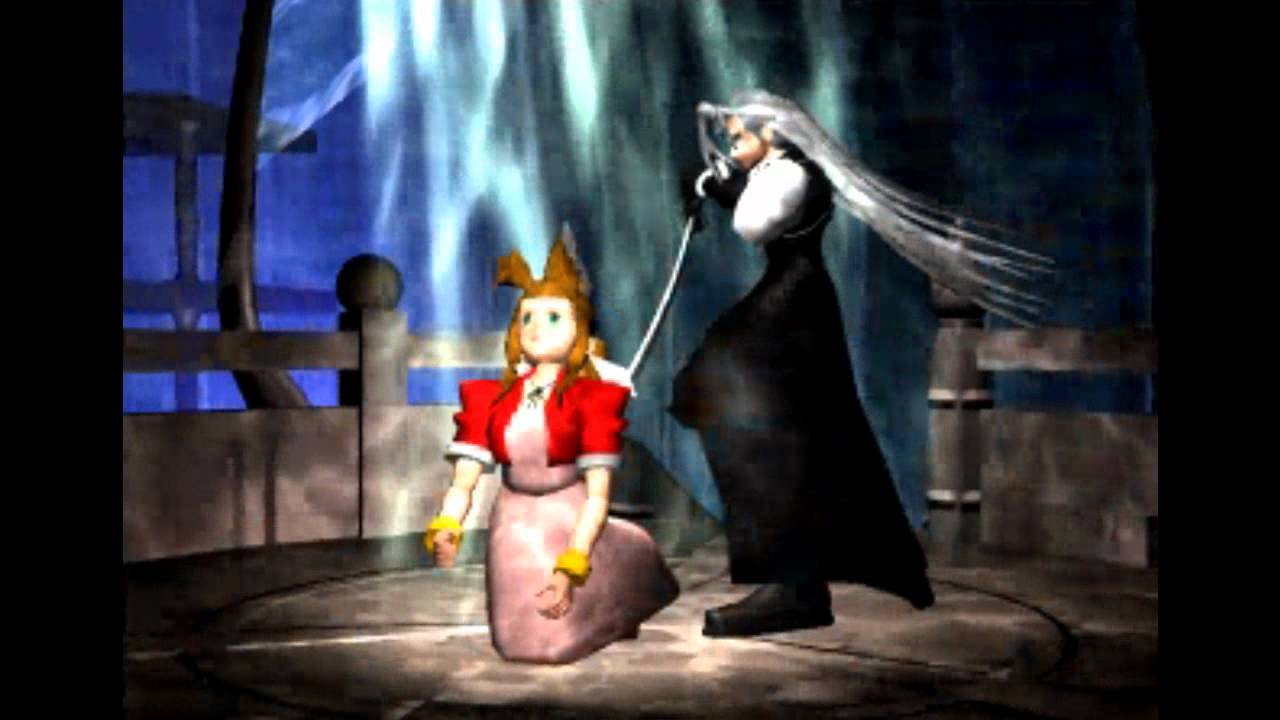
\includegraphics[width=90mm]{maxresdefault.jpg}
\caption{Final Fantasy 7 Aerith Death Cutscene \label{overflow}}
\label{fig:FF7}
\end{figure}
Clearly, the ability to invoke emotion is not something that can be measured using surface roughness or other such technical metrics. Storytelling is an essential aspect in creating an immersive experience. However, there are many games without plots that also offer a highly immersive experience for players. One such game is Minecraft, which offers players a 3d sandbox environment in which they must survive in a hostile world while building and exploring a procedurally generated voxel world containing caves mountains and countless other environments. This game features relatively primitive shaders and lighting effects and has a very minimal plot and few NPCs, yet the game still offers a highly immersive and addictive player experience. Players denote thousands of hours to building detailed and complex structures within the game world and express genuine stress and unease when faced with the in-game monsters, despite their unrealistic appearances. \cite{fig:MCmonster} 
\begin{figure}[ht!]
\centering
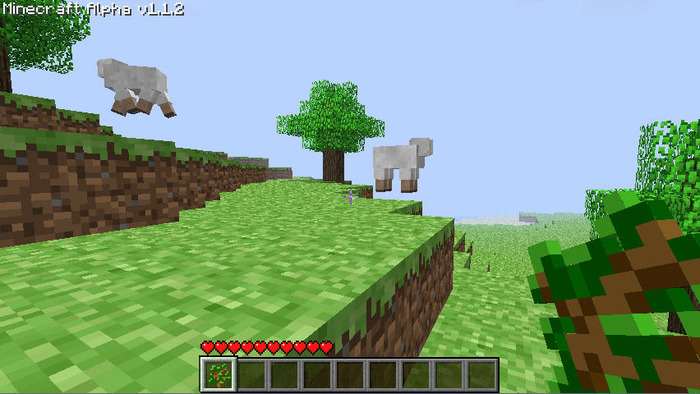
\includegraphics[width=90mm]{minecraft-32.jpg}
\caption{Minecraft Gameplay \label{overflow}}
\label{fig:Minecraft}
\end{figure}
\cite{fig:MCmonster} 
\begin{figure}[ht!]
\centering
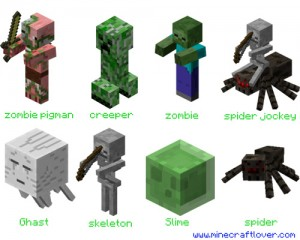
\includegraphics[width=90mm]{minecraft-spider-300x240.jpg}
\caption{Minecraft Hostile NPCs (source: http://www.minecraftlover.com) \label{overflow}}
\label{fig:MCmonster}
\end{figure}
A game's capacity to elicit an emotional response in the user is an essential and undeniable factor in its immersive qualities. We argue for  
\section[My new section]{An example of making a new section and giving it a short name}\label{sec:newsec}

The \ic{chapter} and \ic{subsection} commands work in exactly the same manner. Each new chapter must have \texttt{$\backslash$chapter[short name]\{chapter name\}} as its first line.

``Hey, wait a minute. What if I need to refer to that section? How can I do that?'' It's actually as simple as adding\verb+\label{labelname}+ at the end of the \ic{chapter} command like\texttt{$\backslash$section[My new section]\{An example of making a new section and giving it a short name\}$\backslash$label\{sec:newsec\}}. Now I can refer to Section \ref{sec:newsec} by typing \verb+\ref{sec:newsec}+. You can label just about anything and refer to the label to get an automatically generated number for the item. This means that you need to come up with a labeling scheme before you start writing and stick with it.

Some other things you'll need to be able to do include italicizing and bolding text and creating lists. These are also easy to accomplish. For example I can use \ic{emph} or \ic{textit} to italicize text. To italicize homework I would enter \verb|\emph{homework}| or \verb|\textit{homework}| to produce \textit{homework}. To obtain \textbf{bold} text you would use the \ic{textbf} command. And what about lists?

There are several kinds of lists\index{lists} (enumerated, itemized, and descriptive) and each has its own place and environment. An enumerated\index{lists!enumerated} list is good for outlining or ordered lists:

\begin{singlespace}
\begin{example}
\begin{enumerate}
\item First main idea
\begin{enumerate}
\item First subpoint
\item\label{enum:1b} Second subpoint
\end{enumerate}
\item Second main idea
\end{enumerate}
\end{example}
\end{singlespace}

The itemized\index{lists!itemized} list is good for unordered lists or bullet points:

\begin{singlespace}
\begin{example}
\begin{itemize}
\item Idea
\item Idea
\item Idea
\item Idea
\end{itemize}
\end{example}
\end{singlespace}

And the descriptive\index{lists!descriptive} list is good for definitions; however, \ip{amsthm} already has a definition environment, and you will most likely not need the description environment. In any event, here is an example:

\begin{singlespace}
\begin{example}
\begin{description}
\item[First item:] Idea
\item[Second item:] Idea
\item[Third item:] Idea
\end{description}
\end{example}
\end{singlespace}

Notice the use of brackets in the last example. The brackets are optional and the text in the brackets is used as the label for the item. You should also note that you can label an item for later reference see \ref{enum:1b}. There are several options for changing the format of the list environments and a package, \ip{paralist}, for customizing lists which are described in section 3.3 of \citet{mgbcr04}.

\section{Theorems, definitions, examples, oh my!}
The next thing you'll probably need to do is enter definitions, theorems, and examples. Below you will find some examples. On the left you will see the text typed into the document and on the right what it looks like when formatted. These examples are intended to give you a sense of what type of mathematical expressions \lt handles. You should look at Appendix~\ref{math} for a more complete discussion of entering mathematics. In the beginning you will not know all of the commands that you need to enter. Don't worry. Each of the suggested editors has a palette that shows you a picture of what you want and puts the correct commands into the document when you click the picture. As you look at these examples, keep it in mind that some of them use some user defined commands which can be found in \verb|styles/personal.tex|. Now lets look at Definition~\ref{def1} \ref{bdef1}, Theorem~\ref{introwatthm}, and equation~\ref{m.1diasumtwo}.

\begin{singlespace}
\begin{example}
\begin{defn}[One of Ramanujan's
 third order mock theta 
 functions]\label{def1}
 \begin{equation}\label{introf(q)} 
 f(q)=1+\sum_{y=1}^{\infty}
 \frac{q^{y^2}}{(1+q)^2(1+q^2)^2
 \cdots (1+q^y)^2}.
 \end{equation}\end{defn}
\end{example}
\end{singlespace}

\begin{singlespace}
\begin{example}
\begin{thm}[Watson's 
transformation of 
$f(q)$]\label{introwatthm}
\begin{equation}\label{introf}
\qrfac{q}{\infty}
\sum_{y=0}^{\infty} q^{y^2}
 \qrfac[-2]{- q}{y}=1+
 \sum_{y=1}^{\infty}
 \frac{(-1)^{y}
 4q^{(3/2)y^2+
 (1/2)y}}{(1+q^{y})}.
 \end{equation}\end{thm}
\end{example}
\end{singlespace}

This is a more complicated example which uses the \ic{substack} command to have multiple summation criteria.
\begin{singlespace}
\begin{example}
\begin{align}\label{m.1diasumtwo}
\left[NUM\right]_1^{(\fl)}(q;b;
\bvec{x})=&\ q\sum\limits_{
\substack{ 0\leq r,t 
\leq\fl-1}}
q^{r+t}\sum\limits_
 {\substack{{\lambda
 \vdash (r+t)}\\
  \lambda/1^r\in V_t\\
  \ell(\lambda)\leq \fl-1}}
  \mathrm{s}_{(b,\lambda)}
  (\bvec{x}).\end{align}
\end{example}
\end{singlespace}

Another thing that one might need to do is create piecewise definitions. This can be accomplished by using the \verb|cases| \index{cases@\verb+cases+} environment. This example also uses the \ic{intertext} command to put text between displayed equations.
\begin{singlespace}
\begin{example}\begin{subequations}\label{2c1BP}
\begin{alignat}{2}\label{2c1BPa} 
A_{y_1}:=&\begin{cases}
 1 &\text{for $y_1=0$},\\
\frac{-1)^{y_1}
4q^{y_1}q^{\binom{y_1}{2}}}
{\qrfac{q}{2y_1}(1+q^{y_1})}
&\text{for $y_1>0$}\end{cases}\\
\intertext{and} B_{y_1}:=&
\qrfac[-1]{-q}{y_1}\qrfac[-1]
{-q}{y_1}=\qrfac[-2]{-q}{y_1}
&.\label{2c1BPb}\end{alignat}
\end{subequations}
\end{example}
\end{singlespace}

Finally, if you need to incorporate examples into your thesis you can do it using the example environment, as seen in Example~\ref{ex:ex}.
\begin{singlespace}
\begin{example}
\begin{ex}[An example example]
\label{ex:ex}
This is an example of including an
 example. Kind of silly isn't it.
 \end{ex}
\end{example}
\end{singlespace}

\section{Putting code in the main body of the thesis}
There is one last textual item which Computer Science majors and probably some Mathematics majors will need to incorporate, pseudocode\index{pseudocode}. To do this I would suggest using the \ic{lstlisting} environment. Below is an example set up for the \ip{listings} package. You could put your modifications to this set up into the \texttt{personal.tex} file in the \texttt{styles} folder. Documentation on the \ip{listings} package can be found in the \texttt{doc} folder with the documentation for the other packages.
\lstset{
               language =Pascal, % pick a language style
               emph={return,natural, numbers, integers, increasing},
               emphstyle={\bfseries},% choose other keywords and a format
               linewidth=.95\textwidth, breaklines=true, commentstyle=\textit,
               stringstyle=\upshape, showspaces=false, numbers=left,
               numberstyle=\tiny, basicstyle=\small, xleftmargin=30pt,
               breakautoindent=true, captionpos=b
               }
{\small\begin{singlespace}
\begin{verbatim}
\lstset{
        language =Pascal, % pick a language style
        emph={return,natural, numbers, integers, increasing},
        emphstyle={\bfseries},% choose other keywords and a format
        linewidth=.95{\textwidth}, breaklines=true,commentstyle=\textit,
        stringstyle=\upshape,showspaces=false,numbers=left,
        numberstyle=\tiny,basicstyle=\small,xleftmargin=30pt,
        breakautoindent=true,captionpos=b
        }
\end{verbatim}
\end{singlespace}}

The listing in Listing~\ref{largesteven} gives an algorithm for finding the largest even integer in a given list of $n$ integers. I have used the \texttt{mathescape}\index{listings!mathescape} option to be able to incorporate mathematics in the listing. The actual code put in the thesis is given first and the formatted output follows.

{\small\begin{singlespace}
\begin{verbatim}
\begin{lstlisting}[mathescape, caption= Find the location 
of the largest even integer in a list,label=largesteven]
procedure $largestevenlocation$($a_1, a_2, \ldots, a_n$: integers)
$k$:=0
$largest$:=-$\infty$
for $i$:=1 to $n$
  if ($a_i$ is even and $a_i>largest$) then
  begin
    $k$:=$i$
    $largest$:=$a_i$
  end
end
return $k$
\end{lstlisting}
\end{verbatim}
\end{singlespace}
}
\begin{singlespace}
\begin{lstlisting}[mathescape, caption= Find the location
 of the largest even integer in a list,label=largesteven]
procedure $largestevenlocation$($a_1, a_2, \ldots, a_n$: integers)
$k$:=0
$largest$:=-$\infty$
for $i$:=1 to $n$
  if ($a_i$ is even and $a_i>largest$) then
  begin
    $k$:=$i$
    $largest$:=$a_i$
  end
end
return $k$
\end{lstlisting}
\end{singlespace}
The code in Listing~\ref{quartsearch} is an improvement on Binary search. The algorithm reduces the size of the search by a factor of four at each iteration. It provides another example of using the \ic{lstlisting} environment.
\begin{singlespace}\small
\begin{verbatim}
\begin{lstlisting}[mathescape,caption=Quartary search,
label=quartsearch]
procedure $quartarysearch$($x$: integer, $a_1, a_2,
 \ldots, a_n$: increasing integers)
$i$:=$1$
$j$:=$n$
while $i<j-2$
begin
  $l:=\lfloor(i+j)/4\rfloor$
  $m:=\lfloor(i+j)/2\rfloor$
  $u:=\lfloor3(i+j)/4\rfloor$
  if $x>a_m$ then
    if $x\leq a_u$ then
    begin
      $i:=m+1$
      $j:=u$
    end
    else
     $i:=u+1$
  else if $x>a_l$ then
    begin
      $i:=l+1$
      $j:=m$
    end
    else $j:=l$
end
if $x=a_i$ then $location:= i$
else if $x=a_j$ then $location:= j$
else if $x=a_{\lfloor(i+j)/2\rfloor}$ then
 $location:= \lfloor(i+j)/2\rfloor$
else $location:= 0$
return $location$
\end{lstlisting}
\end{verbatim}
\end{singlespace}
\begin{singlespace}
\begin{lstlisting}[mathescape,caption=Quartary search,label=quartsearch]
procedure $quartarysearch$($x$: integer, $a_1, a_2, \ldots, a_n$: increasing integers)
$i$:=$1$
$j$:=$n$
while $i<j-2$
begin
  $l:=\lfloor(i+j)/4\rfloor$
  $m:=\lfloor(i+j)/2\rfloor$
  $u:=\lfloor3(i+j)/4\rfloor$
  if $x>a_m$ then
    if $x\leq a_u$ then
    begin
      $i:=m+1$
      $j:=u$
    end
    else
     $i:=u+1$
  else if $x>a_l$ then
    begin
      $i:=l+1$
      $j:=m$
    end
    else $j:=l$
end
if $x=a_i$ then $location:= i$
else if $x=a_j$ then $location:= j$
else if $x=a_{\lfloor(i+j)/2\rfloor}$ then $location:= \lfloor(i+j)/2\rfloor$
else $location:= 0$
return $location$
\end{lstlisting}
\end{singlespace}

\section{What is in \texttt{username.tex}}
Before we move on let's talk a little bit about what is at the beginning of \verb|username.tex|. The file starts with 
\verb|\documentclass{woosterthesis}|, which must be at the beginning of every IS. In the brackets are options for the woosterthesis class. The options are the same as for the \verb|book| class with some additional options  \verb|abstractonly|\index{woosterthesis options!abstractonly}, \verb|alltt|\index{woosterthesis options!alltt},  \verb|blacklinks|\index{woosterthesis options!blacklinks}, \verb|code|\index{woosterthesis options!code}, \verb|dropcaps|\index{woosterthesis options!dropcaps}, \verb|euler|\index{woosterthesis options!euler}, \verb|guass|\index{woosterthesis options!guass}, 
\verb|index|\index{woosterthesis options!index}, \verb|kaukecopyright|\index{woosterthesis options!kaukecopyright}, \verb|palatino|\index{woosterthesis options!palatino}, \verb|picins|\index{woosterthesis options!picins}, \verb|verbatim|\index{woosterthesis options!verbatim}, and \verb|xetex|\index{woosterthesis options!xetex}. The \verb|kaukecopyright| option will put the arch symbol with the word mark on the copyright page. The \verb|blacklinks| option will make the hyperlinks in the PDF version of the thesis black and suitable for printing; normally the links are colored to provide visual clues to the reader.  The \verb|code| option will use \ip{listings} style to format program code examples.  The \verb|abstractonly| option will allow you to print just the Abstract. The \verb|palatino| option will use the \ip{pxfonts} package which uses the Palatino fonts. The \verb|picins| option will use the \ip{floatflt} package to allow text to wrap around images. \verb|index| will allow the \ip{makeidx} package to be loaded so that if you have index entries they will be added to an index (this reqires additional steps). \verb|dropcaps| loads the \ip{letterine} package for doing dropped capitals and \verb|alltt| loads the \ip{alltt} for using typewriter type in various ways. \verb|verbatim| allows one to set verbatim what is entered. \verb|euler| and \verb|guass| load the \ip{woofncychap} package with the named option which will change the look of chapter headings. Finally \verb|xetex| will allow you to use the \ifthenelse{\boolean{xetex}}{\XeTeX\ }{XeTeX} extension of \TeX{} for easy use of system fonts. Adding or deleting options from the comma separated list will change the appearance of the document and some options should only be used after consulting your advisor. Now let's move on to some other things that you'll need to deal with: figures, pictures, and tables.

%!TEX root = ../username.tex
\chapter{Working with figures and tables}\label{graphics}

\section{Getting a simple figure in the document}
In this chapter we want to talk about including figures and tables in the document. To insert a simple figure you can enter something like
\begin{singlespace}\small
\begin{verbatim}
\begin{figure}[!ht]
\begin{center}
\woopic{picture3}{.8}
\end{center}
\caption{Our first
 picture}\label{first}
\end{figure}
\end{verbatim}
\end{singlespace}
\vspace{-2 in}
\begin{figure}[!ht]
\rightline{
\begin{minipage}{.5\textwidth}
\begin{center}
\woopic{picture3}{.8}
\vspace{-.5 in}
\caption{Our first picture}\label{first}
\end{center}
\end{minipage}
}
\end{figure}

The \verb|!ht| tell \LaTeX{} to try and place the figure here no matter what or at the top of the next page. The \verb|\woopic| command takes the name of the picture as the first argument and the scaling factor as the second argument. The scaling factor must be between zero and one and the figure name must have \emph{no spaces}. Your figures can be in one of three formats: jpg, tif, or pdf. Captions are placed below the figure and your label should be placed after the caption.

In the next example we are using the woosterthesis option \verb|picins|\index{woosterthesis options!picins} to typeset a picture inside a paragraph and have the text wrap around the figure. This option loads the \ip{wrapfig} package. One thing to note is that the figures placed in this manner do not float with the other figures and as such numbering could get out of sequence. Keep an eye out for such behavior.  This technique should be used sparingly in your thesis.

\begin{singlespace}\small
\begin{verbatim}
\newcommand{\sample}{Some text that is reused over and over
 again in the example. }
\begin{wrapfigure}{r}{2.2in}
\woopic{picture2}{.4}
\caption{Conchoid.}
\end{wrapfigure}
\sample\sample\sample\sample
\end{verbatim}
\end{singlespace}

\newcommand{\sample}{Some text that is reused over and over again in the example. }
\begin{wrapfigure}{r}{2.2in}
\woopic{picture2}{.4}
\caption{Conchoid.}
\end{wrapfigure}
\sample\sample\sample\sample\sample\sample\sample\sample\sample


\subsection{Minipages}

You can also create minipages in your documents to accomplish more complicated formatting. For example you could try the following which produces Figure~\ref{Fig2}.
\begin{singlespace}\small
\begin{verbatim}
\begin{minipage}[t][3 in][t]{1 in}
This is a minipage which is 3 in tall and 1 in wide.
 Top Text Text Text Text.\end{minipage}\hfill
\begin{minipage}[t][3 in][c]{1 in}
This is a minipage which is 3 in tall and 1 in wide.
 Center Text Text Text Text.\end{minipage}\hfill
\begin{minipage}[t][3 in][b]{1 in}
This is a minipage which is 3 in tall and 1 in wide.
 Bottom Text Text Text Text.\end{minipage}
\end{verbatim}
\end{singlespace}

\begin{figure}[!htb]
\begin{minipage}[t][3 in][t]{1 in}
This is a minipage which is 3 in tall and 1 in wide. Top Text Text Text Text.
\end{minipage}
\hfill
\begin{minipage}[t][3 in][c]{1 in} This is a minipage which is 3 in tall and 1 in wide. Center Text Text Text Text.
\end{minipage}
\hfill
\begin{minipage}[t][3 in][b]{1 in}
This is a minipage which is 3 in tall and 1 in wide. Bottom Text Text Text Text.
\end{minipage}
\caption{Minipage example}\label{Fig2}
\end{figure}

In the example above, the syntax \verb|\begin{minipage}[t][3 in][t]{1 in}| follows the convention \linebreak\verb|\begin{minipage}[minipageposition][height][textposition]{width}|\index{minipage}

\subsubsection[Two pictures in one figure]{How to get more than one picture in the same figure}

You can use minipages to put more than one picture in a figure. Here is an example of how to do this.
\begin{singlespace}\small
\begin{verbatim}
\begin{minipage}[!ht]{6cm}
\woopic{picture1}{.4}
\par
\caption[What goes in the List of Figures]{Left}
\end{minipage}
\hfill
\begin{minipage}[!ht]{6cm}
\woopic{picture2}{.4}
\end{picture}\par
\caption{Right}
\end{minipage}
\end{verbatim}
\end{singlespace}
\begin{figure}[!ht]
\begin{minipage}[!ht]{6cm}
\woopic{picture1}{.4}
\par
\caption[What goes in the List of Figures]{Left}
\end{minipage}
\hfill
\begin{minipage}[!ht]{6cm}
\woopic{picture2}{.4}
\par
\caption{Right}
\end{minipage}
\end{figure}

You can also use the \ip{subfigure} package to do this.

\begin{singlespace}\small
\begin{verbatim}
\begin{figure}[!ht]\centering
\subfigure[What goes in the List][Large conchoid]
{\woopic{picture1}{.4}\label{fig3:left}}
\qquad
\subfigure[What goes in the List][Small conchoid]
{\woopic{picture2}{.4}\label{fig3:right}}
\caption{Two pictures in one figure}\label{fig3}
\end{figure}
\end{verbatim}
\end{singlespace}
\begin{figure}[!ht]\centering
\subfigure[What goes in the List][Large conchoid]
{\woopic{picture1}{.4}\label{fig3:left}}
\qquad
\subfigure[What goes in the List][Small conchoid]
{\woopic{picture2}{.4}\label{fig3:right}}
\caption{Two pictures in one figure}\label{fig3}
\end{figure}

We should now be able to refer to either Figure~\ref{fig3}~\subref{fig3:left} or Figure~\ref{fig3}~\subref{fig3:right} using the labels we gave to the left and right images.

The reader is referred to Chapters 8, 9, and 16 of \citet{kd03} or to Chapters 6 and 10 of \citet{mgbcr04} for a complete discussion of figures and graphics.

\section{Tables}

Tables are fairly easy to set up. Here is a simple table
\begin{singlespace}\small
\begin{verbatim}
\begin{table}[!ht]
\begin{center}
\begin{tabular}{r l}
  $\underline{\textnormal{District}}$ &  
  $\underline{\textnormal{Population}}$\\
   Applewood & 8280 \\
   Boxwood & 4600  \\
   Central & 5220
   \end{tabular}\caption{Our first table}
   \end{center}
\end{table}
\end{verbatim}
\end{singlespace}
\begin{table}[!ht]
\begin{center}
\begin{tabular}{r l}
  $\underline{\textnormal{District}}$ &
    $\underline{\textnormal{Population}}$\\
   Applewood & 8280 \\
   Boxwood & 4600  \\
   Central & 5220
   \end{tabular}\caption{Our first table}
   \end{center}
\end{table}

In \verb|\begin{tabular}{r l}| the two ``r'' and ``l'' indicate that we have two columns with right and left aligned entries and no lines dividing cells or around the table. I can make the table look more like a spreadsheet by doing
\begin{singlespace}\small
\begin{verbatim}
\begin{table}[!ht]
\begin{center}
\begin{tabular}{|r|l|}
\hline
  {\textnormal{District}} &  
  {\textnormal{Population}}\\ \hline
   Applewood & 8280 \\ \hline
   Boxwood & 4600  \\ \hline
   Central & 5220\\ \hline
   \end{tabular}\caption{Our first table again}
   \end{center}
\end{table}
\end{verbatim}
\end{singlespace}
\begin{table}[!ht]
\begin{center}
\begin{tabular}{|r|l|}
\hline
  {\textnormal{District}} &  
  {\textnormal{Population}}\\ \hline
   Applewood & 8280 \\ \hline
   Boxwood & 4600  \\ \hline
   Central & 5220\\ \hline
   \end{tabular}\caption{Our first table again}
   \end{center}
\end{table}

Here is a more complicated example of a table.
\begin{singlespace}\small
\begin{verbatim}
\begin{table}[!ht]
\centerline{
\begin{tabular}{|l||r|r|r|r|} \hline
\emph{Reprojection} & \multicolumn{3}{|c|}{\emph{Largest
 Reduction of Curvature}}
  & \emph{Average} \\ \cline{2-4}
\emph{Method} & \emph{Original} & \emph{Reprojected} &
 \emph{at} & 
  \emph{Reduction} \\ 
 & \emph{Curvature} & \emph{Curvature} &
  \emph{Rotation} & \emph{of Curvature} \\ 
  \hline \hline
ZEEL & 0.0358 & 0.0245 &
 $\degree{45}$ & 0.0050 \\ \hline
ZEEL ext.\ & 0.0358 & 0.0245 &
 $\degree{45}$ & 0.0059 \\ \hline
Regridding & 0.0428 & 0.0166 &
 $\degree{75}$ & 0.0159 \\ \hline
Block & 0.0358 & 0.0103 &
 $\degree{45}$ & 0.0163 \\ \hline
\end{tabular}}
\caption{Reduction of curvature by each
 reprojection method\label{tbl:kreduce}}
\end{table}
\end{verbatim}
\end{singlespace}
\begin{table}[!ht]
\centerline{
\begin{tabular}{|l||r|r|r|r|} \hline
\emph{Reprojection} & \multicolumn{3}{|c|}{\emph{Largest Reduction of Curvature}} 
  & \emph{Average} \\ \cline{2-4}
\emph{Method} & \emph{Original} & \emph{Reprojected} & \emph{at} & 
  \emph{Reduction} \\ 
 & \emph{Curvature} & \emph{Curvature} & \emph{Rotation} & \emph{of Curvature} \\ 
  \hline \hline
ZEEL & 0.0358 & 0.0245 & $\degree{45}$ & 0.0050 \\ \hline
ZEEL ext.\ & 0.0358 & 0.0245 & $\degree{45}$ & 0.0059 \\ \hline
Regridding & 0.0428 & 0.0166 & $\degree{75}$ & 0.0159 \\ \hline
Block & 0.0358 & 0.0103 & $\degree{45}$ & 0.0163 \\ \hline
\end{tabular}}
\caption{Reduction of curvature by each reprojection method\label{tbl:kreduce}}
\end{table}

Please refer to Chapter 6 of \citet{kd03} for a complete discussion of tables and tabular environments.


%!TEX root = ../username.tex
\chapter{Working with bibliographies and indicies}\label{bibind}
I would highly recommend that you use Bib\TeX{} to create your bibliography. Bib\TeX{} processes a special .bib file. The .bib file is where you enter your bibliographic information. A sample entry looks something like
\begin{singlespace}\small
\begin{verbatim}
@article{feu02,
author=		{Thomas~Feuerstack},
title=			{Introduction to pdf{\TeX{}}}, 
journal=		{TUGboat}, 
volume=		{23},
pages=		{329--334},
number=		{3/4},
url=			{http://www.tug.org/TUGboat/Articles/tb23-3-4/tb75feu.pdf},
year=			2002}
\end{verbatim}
\end{singlespace}
or
\begin{singlespace}\small
\begin{verbatim}
@book{mgbcr04,
author=			{Frank~Mittelbach and Michel~Goossens and
Johannes~Braams and David~Carlisle and Chris~Rowley},
title=				{The \LaTeX\ Companion},
publisher=			{Addison Wesley Professional},
edition=			{2nd},
address=			{New York},
year=				2004}
\end{verbatim}
\end{singlespace}

For a Web site I would recommend the following
\begin{singlespace}\small
\begin{verbatim}
@misc{brei04,
author = 			{Jon~Breitenbucher},
title = 				{{W}ooster related {L}a{T}e{X} files},
url = 				{http://jbreitenbuch.wooster.edu/~jonb/latex/},
howpublished=	{World Wide Web},
year=				2004,
note = 			{Accessed on 03/11/2004}}
\end{verbatim}
\end{singlespace}

You can make a reference by typing \verb|\citet{mgbcr04}| to produce \citet{mgbcr04}. Other forms for citation include \verb|\citep{mgbcr04}| or  \verb|\citeauthor| \verb|{mgbcr04}| to produce \citep{mgbcr04} or \citeauthor{mgbcr04} respectively. You can consult \citet{kd03} or \citet{mgbcr04} to find out how to format entries in the .bib file and what options each reference type has.\footnote{You could also use footnotes if your department called for that.}

Indicies are also relatively easy to create. If I wanted to have Wooster\index{Wooster} show up in the index, I would enter \verb|Wooster\index{Wooster}| in my source file. I could create a subentry for User Services\index{Wooster!User Services} by entering \verb|User Services|\verb|\index{Wooster!User Services}|. A subsubentry for Help Desk\index{Wooster!User Services!Help Desk} would be entered as \verb|\index{Wooster!User| \verb|Services!Help Desk}|.

To create the index one needs to make sure to uncomment the \verb|\makeindex| command in the \texttt{username.tex} file. One also needs to uncomment the makeidx entry in the \verb|styles/packages.tex| file and then run the Makeindex program. Consult \citet{kd03} or \citet{mgbcr04} for further information.
%\input{chapters/chapter4}
%\input{chapters/chapter5}
%\input{chapters/chapter6}
%\input{chapters/chapter7}
%\input{conclusion}

%%%%%%%%%%%%%%%%%%%%%%%%%%%%%%%%%%%%%%%%%%%%%%%%%%%%%%%%%%%%%%%%%%%%%%%%%%%%%%%%%%%%%%%%%%%%%%
% This section starts the back matter. The back matter includes appendices, indicies, and the %bibliography
%%%%%%%%%%%%%%%%%%%%%%%%%%%%%%%%%%%%%%%%%%%%%%%%%%%%%%%%%%%%%%%%%%%%%%%%%%%%%%%%%%%%%%%%%%%%%%

\backmatter

%%!TEX root = ../username.tex
%%%%%%%%%%%%%%%%%%%%%%%%%%%%%%%%%%%%%%%%%%%%%%%%%%%%%%%%%%%%%%%%
% Contents: Math typesetting with LaTeX
% $Id: math.tex,v 1.3 2005/05/21 02:03:43 jonb Exp $
%%%%%%%%%%%%%%%%%%%%%%%%%%%%%%%%%%%%%%%%%%%%%%%%%%%%%%%%%%%%%%%%%

\chapter{Typesetting Mathematical Formulae}\label{math}
\begin{intro}
  This appendix is taken from \citet{ophs03} under the GNU open source documentation license. This appendix addresses the main strength
  of \TeX{}: mathematical typesetting. But be warned, this appendix
  only scratches the surface. While the things explained here are
  sufficient for many people, don't despair if you can't find a
  solution to your mathematical typesetting needs here. It is highly likely
  that your problem is addressed in \AmS-\LaTeX{}%
  \footnote{\texttt{CTAN:/tex-archive/macros/latex/packages/amslatex}}
  or some other package.
\end{intro}
  
\section{General}

\LaTeX{} has a special mode for typesetting mathematics\index{mathematics}.
Mathematical text within a paragraph is entered between \verb|\(|\index{\(@\verb+\(+}
and \verb|\)|\index{\)@\verb+\)+}, %$
between \texttt{\$} and \texttt{\$} or between
\verb|\begin{|{math}\verb|}| and \verb|\end{math}|.\index{formulae}

\begin{singlespace}
\begin{example}
Add $a$ squared and $b$ squared 
to get $c$ squared. Or, using 
a more mathematical approach:
$c^{2}=a^{2}+b^{2}$
\end{example}
\end{singlespace}

\begin{singlespace}
\begin{example}
\TeX{} is pronounced as 
$\tau\epsilon$.\\[6pt]
100~m$^{3}$ of water\\[6pt]
This comes from my $\heartsuit$
\end{example}
\end{singlespace}

It is preferable to \emph{display} larger mathematical equations or formulae,
rather than to typeset them on separate lines. This means you enclose them
in \verb|\[| \index{\[@\verb+\[+} and \verb|\]| \index{\]@\verb+\]+} or between
\verb|\begin{|displaymath\index{displaymath}\verb|}| and
  \verb|\end{displaymath}|.  This produces formulae which are not
numbered. If you want \LaTeX{} to number them, you can use the
equation\index{equation} environment.


\begin{singlespace}
\begin{example}
Add $a$ squared and $b$ squared 
to get $c$ squared. Or, using 
a more mathematical approach:
\begin{displaymath}
c^{2}=a^{2}+b^{2}
\end{displaymath}
And just one more line.
\end{example}
\end{singlespace}

You can reference an equation with \ic{label} and \ic{ref}

\begin{singlespace}
\begin{example}
\begin{equation} \label{eq:eps}
\epsilon > 0
\end{equation}
From (\ref{eq:eps}), we gather 
\ldots
\end{example}
\end{singlespace}

Note that expressions will be typeset in a different style if displayed:

\begin{singlespace}
\begin{example}
$\lim_{n \to \infty} 
\sum_{k=1}^n \frac{1}{k^2} 
= \frac{\pi^2}{6}$
\end{example}
\end{singlespace}
\begin{singlespace}
\begin{example}
\begin{displaymath}
\lim_{n \to \infty} 
\sum_{k=1}^n \frac{1}{k^2} 
= \frac{\pi^2}{6}
\end{displaymath}
\end{example}
\end{singlespace}

There are differences between \emph{math mode} and \emph{text mode}. For
example in \emph{math mode}: 

\begin{enumerate}

\item Most spaces and linebreaks do not have any significance, as all spaces
either are derived logically from the mathematical expressions or
have to be specified using special commands such as \verb|\,| \index{''\,@\verb+\,+}, \ic{quad}, or \ic{qquad}.
 
\item Empty lines are not allowed. Only one paragraph per formula.

\item Each letter is considered to be the name of a variable and will be
typeset as such. If you want to typeset normal text within a formula
(normal upright font and normal spacing) then you have to enter the
text using the \verb|\textrm{...}| commands.
\end{enumerate}


\begin{singlespace}
\begin{example}
\begin{equation}
\forall x \in \mathbf{R}:
\qquad x^{2} \geq 0
\end{equation}
\end{example}
\end{singlespace}

\begin{singlespace}
\begin{example}
\begin{equation}
x^{2} \geq 0\qquad
\textrm{for all }x\in\mathbf{R}
\end{equation}
\end{example}
\end{singlespace}

Mathematicians can be very fussy about which symbols are used:
it would be conventional here to use `blackboard bold\index{blackboard bold}',
bold symbols\index{bold symbols} which is obtained using \ic{mathbb} from the
package \ip{amsfonts} or \ip{amssymb}.

\ifx\mathbb\undefined\else
The last example becomes
\begin{singlespace}
\begin{example}
\begin{displaymath}
x^{2} \geq 0\qquad
\textrm{for all }x\in\mathbb{R}
\end{displaymath}
\end{example}
\end{singlespace}
\fi

\section{Grouping in Math Mode}

Most math mode commands act only on the next character. So if you
want a command to affect several characters, you have to group them
together using curly braces: \verb|{...}|.

\begin{singlespace}
\begin{example}
\begin{equation}
a^x+y \neq a^{x+y}
\end{equation}
\end{example}
\end{singlespace}
 
\section{Building Blocks of a Mathematical Formula}

In this section, the most important commands used in mathematical
typesetting will be described. Take a look at \citet{kd03} for a detailed list of commands for typesetting
mathematical symbols.

\textbf{Lowercase Greek letters\index{Greek letters}} are entered as \verb|\alpha|,
 \verb|\beta|, \verb|\gamma|, \ldots, uppercase letters
are entered as \verb|\Gamma|, \verb|\Delta|, \ldots\footnote{There is no
  uppercase Alpha defined in \LaTeXe{} because it looks the same as a
  normal roman A. Once the new math coding is done, things will
  change.} 

\begin{singlespace}
\begin{example}
$\lambda,\xi,\pi,\mu,\Phi,\Omega$
\end{example}
\end{singlespace}
 
\textbf{Exponents and Subscripts} can be specified using\index{exponent}\index{subscript}
the \verb|^|\index{^@\verb+^+} and the \verb|_|\index{_@\verb+_+} character.

\begin{singlespace}
\begin{example}
$a_{1}$ \qquad $x^{2}$ \qquad
$e^{-\alpha t}$ \qquad
$a^{3}_{ij}$\\
$e^{x^2} \neq {e^x}^2$
\end{example}
\end{singlespace}

The \textbf{square root\index{square root}} is entered as \ic{sqrt}, the
$n^\mathrm{th}$ root is generated with \verb|\sqrt[|$n$\verb|]|. The size of
the root sign is determined automatically by \LaTeX. If just the sign
is needed, use \ic{surd}.

\begin{singlespace}
\begin{example}
$\sqrt{x}$ \qquad 
$\sqrt{ x^{2}+\sqrt{y} }$ 
\qquad $\sqrt[3]{2}$\\[3pt]
$\surd[x^2 + y^2]$
\end{example}
\end{singlespace}

The commands \ic{overline} and \ic{underline} create
\textbf{horizontal lines} directly over or under an expression.
\index{horizontal!line}

\begin{singlespace}
\begin{example}
$\overline{m+n}$
\end{example}
\end{singlespace}

The commands \ic{overbrace} and \ic{underbrace} create
long \textbf{horizontal braces} over or under an expression.
\index{horizontal!brace}

\begin{singlespace}
\begin{example}
$\underbrace{ a+b+\cdots+z }_{26}$
\end{example}
\end{singlespace}

\index{mathematical!accents} To add mathematical accents such as small
arrows or {tilde} signs to variables, you can use the commands
given in \citet{kd03}.  Wide hats and
tildes covering several characters are generated with \ic{widetilde}
and \ic{widehat}.  The \verb|'|\index{'@\verb+'+} symbol gives a
prime\index{prime}.
% a dash is --

\begin{singlespace}
\begin{example}
\begin{displaymath}
y=x^{2}\qquad y'=2x\qquad y''=2
\end{displaymath}
\end{example}
\end{singlespace}

\textbf{Vectors}\index{vectors} often are specified by adding a small
arrow symbol\index{arrow symbols} on top of a variable. This is done with the
\ic{vec} command. The two commands \ic{overrightarrow} and
\ic{overleftarrow} are useful to denote the vector from $A$ to $B$.

\begin{singlespace}
\begin{example}
\begin{displaymath}
\vec a\quad\overrightarrow{AB}
\end{displaymath}
\end{example}
\end{singlespace}

Names of log-like functions are often typeset in an upright
font and not in italic like variables. Therefore \LaTeX{} supplies the
following commands to typeset the most important function names:
\index{mathematical!functions}

\begin{singlespace}
\begin{verbatim}
\arccos   \cos    \csc   \exp   \ker     \limsup  \min   \sinh
\arcsin   \cosh   \deg   \gcd   \lg      \ln      \Pr    \sup
\arctan   \cot    \det   \hom   \lim     \log     \sec   \tan
\arg      \coth   \dim   \inf   \liminf  \max     \sin   \tanh
\end{verbatim}
\end{singlespace}

\begin{singlespace}
\begin{example}
\[\lim_{x \rightarrow 0}
\frac{\sin x}{x}=1\]
\end{example}
\end{singlespace}

For the modulo function\index{modulo function}, there are two commands: \ic{bmod} for the
binary operator ``$a \bmod b$'' and \ic{pmod}
for expressions
such as ``$x\equiv a \pmod{b}$.''

A built-up \textbf{fraction\index{fraction}} is typeset with the
\ic{frac}\verb|{...}{...}| command.
Often the slashed form $1/2$ is preferable, because it looks better
for small amounts of `fraction material.'

\begin{singlespace}
\begin{example}
$1\frac{1}{2}$~hours
\begin{displaymath}
\frac{ x^{2} }{ k+1 }\qquad
x^{ \frac{2}{k+1} }\qquad
x^{ 1/2 }
\end{displaymath}
\end{example}
\end{singlespace}

To typeset binomial coefficients or similar structures, you can use
either the command \linebreak \ic{binom}\{\emph{num}\}\{\emph{denom}\} or \ic{genfrac}\{\emph{ldelim}\}\{\emph{rdelim}\}\{\emph{thickness}\}\{\emph{style}\}\{\emph{num}\}\{\emph{denom}\}. The second command can be used to produce customized fraction like output and more information can be found in \citet{mgbcr04}.

\begin{singlespace}
\begin{example}
\begin{displaymath}
\binom{n}{k}\qquad 
\genfrac{}{}{0pt}{}{x}{y+2}
\end{displaymath}
\end{example}
\end{singlespace}
 
\medskip

The \textbf{integral operator\index{integral operator}} is generated with \ic{int}, the
\textbf{sum operator\index{sum operator}} with \ic{sum}. The upper and lower limits
are specified with~\verb|^|\index{^@\verb+^+} and~\verb|_|\index{_@\verb+_+} like subscripts and superscripts.

\begin{singlespace}
\begin{example}
\begin{displaymath}
\sum_{i=1}^{n} \qquad
\int_{0}^{\frac{\pi}{2}} \qquad
\end{displaymath}
\end{example}
\end{singlespace}

For \textbf{braces\index{braces}} and other delimiters\index{delimiters}, there exist all
types of symbols in \TeX{} (e.g.~$[\;\langle\;\|\;\updownarrow$).
Round and square braces can be entered with the corresponding keys,
curly braces with \verb|\{|, all other delimiters are generated with
special commands (e.g.~\verb|\updownarrow|). For a list of all
delimiters available, check \citet{kd03}.

\begin{singlespace}
\begin{example}
\begin{displaymath}
{a,b,c}\neq\{a,b,c\}
\end{displaymath}
\end{example}
\end{singlespace}

If you put the command \ic{left} in front of an opening delimiter or
\ic{right} in front of a closing delimiter, \TeX{} will automatically
determine the correct size of the delimiter. Note that you must close
every \ic{left} with a corresponding \ic{right}, and that the size is
determined correctly only if both are typeset on the same line. If you
don't want anything on the right, use the invisible `\verb|\right .|\index{commands!right@\verb+right .+}'!

\begin{singlespace}
\begin{example}
\begin{displaymath}
1 + \left( \frac{1}{ 1-x^{2} }
    \right) ^3
\end{displaymath}
\end{example}
\end{singlespace}

In some cases it is necessary to specify the correct size of a
mathematical delimiter\index{mathematical!delimiter} by hand,
which can be done using the commands \ic{big}, \ic{Big}, \ic{bigg} and
\ic{Bigg} as prefixes to most delimiter commands.\footnote{These
  commands do not work as expected if a size changing command has been
  used, or the \texttt{11pt} or \texttt{12pt} option has been
  specified.  Use the exscale\index{exscale} or amsmath\index{amsmath} packages to
  correct this behaviour.}

\begin{singlespace}
\begin{example}
$\Big( (x+1) (x-1) \Big) ^{2}$\\
$\big(\Big(\bigg(\Bigg($\quad
$\big\}\Big\}\bigg\}\Bigg\}$\quad
$\big\|\Big\|\bigg\|\Bigg\|$
\end{example}
\end{singlespace}

To enter \textbf{three dots\index{three dots}} into a formula, you can use several
commands. \ic{ldots} typesets the dots on the baseline, \ic{cdots}
sets them centered. Besides that, there are the commands \ic{vdots} for
vertical and \ic{ddots} for diagonal dots\index{diagonal dots}.\index{vertical
  dots}\index{horizontal!dots} You can find another example in section~\ref{sec:vert}.

\begin{singlespace}
\begin{example}
\begin{displaymath}
x_{1},\ldots,x_{n} \qquad
x_{1}+\cdots+x_{n}
\end{displaymath}
\end{example}
\end{singlespace}
 
\section{Math Spacing}

\index{math spacing} If the spaces within formulae chosen by \TeX{}
are not satisfactory, they can be adjusted by inserting special
spacing commands. There are some commands for small spaces: \verb|\,| \index{\,@\verb+\,+} for
$\frac{3}{18}\:\textrm{quad}$ (\demowidth{0.166em}), \verb|\:| \index{\:@\verb+\:+} for $\frac{4}{18}\:
\textrm{quad}$ (\demowidth{0.222em}) and \verb|\;| \index{\;@\verb+\;+} for $\frac{5}{18}\:
\textrm{quad}$ (\demowidth{0.277em}).  The escaped space character
\verb*.\ . generates a medium sized space and \ic{quad}
(\demowidth{1em}) and \ic{qquad} (\demowidth{2em}) produce large
spaces. The size of a quad corresponds to the width of the
character `M' of the current font.  The \verb|\!|\index{"\"!@\texttt{\bs"!}} command produces a
negative space of $-\frac{3}{18}\:\textrm{quad}$ (\demowidth{0.166em}).

\begin{singlespace}
\begin{example}
\newcommand{\rd}{\mathrm{d}}
\begin{displaymath}
\int\!\!\!\int_{D} g(x,y)
  \, \rd x\, \rd y 
\end{displaymath}
instead of 
\begin{displaymath}
\int\int_{D} g(x,y)\rd x \rd y
\end{displaymath}
\end{example}
\end{singlespace}
Note that `d' in the differential is conventionally set in roman.

\AmS-\LaTeX{} provides another way for fine tuning
the spacing between multiple integral signs,
namely the \ic{iint}, \ic{iiint}, \ic{iiiint}, and \ic{idotsint} commands.
With the \ip{amsmath} package loaded, the above example can be
typeset this way:

\begin{singlespace}
\begin{example}
\newcommand{\rd}{\mathrm{d}}
\begin{displaymath}
\iint_{D} \, \rd x \, \rd y
\end{displaymath}
\end{example}
\end{singlespace}

See the electronic document testmath.tex (distributed with
\AmS-\LaTeX) or Chapter 8 of ``The LaTeX Companion''\footnote{
available at \texttt{CTAN:/tex-archive/info/ch8.*}.} for further details.

\section{Vertically Aligned Material}
\label{sec:vert}

To typeset \textbf{arrays}, use the \texttt{array}\index{array} environment. It works
somewhat similar to the \texttt{tabular} environment. The \verb|\\| command is
used to break the lines.

\begin{singlespace}
\begin{example}
\begin{displaymath}
\mathbf{X} =
\left( \begin{array}{ccc}
x_{11} & x_{12} & \ldots \\
x_{21} & x_{22} & \ldots \\
\vdots & \vdots & \ddots
\end{array} \right)
\end{displaymath}
\end{example}
\end{singlespace}

The \texttt{array}\index{array} environment can also be used to typeset expressions which have one
big delimiter by using a ``\verb|.|'' as an invisible right\index{commands!right@\verb+right .+} 
delimiter:

\begin{singlespace}
\begin{example}
\begin{displaymath}
y = \left\{ \begin{array}{ll}
 a & \textrm{if $d>c$}\\
 b+x & \textrm{in the morning}\\
 l & \textrm{all day long}
  \end{array} \right.
\end{displaymath}
\end{example}
\end{singlespace}


For formulae running over several lines or for equation systems\index{equation systems},
you can use the environments \texttt{eqnarray}\index{eqnarray}, and \verb|eqnarray*|
instead of \texttt{equation}. In \texttt{eqnarray} each line gets an
equation number. The \verb|eqnarray*| does not number anything.

The \texttt{eqnarray} and the \verb|eqnarray*| environments work like
a 3-column table of the form \verb|{rcl}|, where the middle column can
be used for the equal sign or the not-equal sign. Or any other sign
you see fit. The \verb|\\| command breaks the lines.

\begin{singlespace}
\begin{example}
\begin{eqnarray}
f(x) & = & \cos x     \\
f'(x) & = & -\sin x   \\
\int_{0}^{x} f(y)dy &
 = & \sin x
\end{eqnarray}
\end{example}
\end{singlespace}

\noindent Notice that the space on either side of the 
the equal signs is rather large. It can be reduced by setting
\verb|\setlength\arraycolsep{2pt}|, as in the next example.

\index{long equations} \textbf{Long equations} will not be
automatically divided into neat bits.  The author has to specify
where to break them and how much to indent. The following two methods
are the most common ones used to achieve this.

\begin{singlespace}
\begin{example}
{\setlength\arraycolsep{2pt}
\begin{eqnarray}\notag
\sin x & = & x -\frac{x^{3}}{3!}
     +\frac{x^{5}}{5!}-{}
                   \\\notag
 & & {}-\frac{x^{7}}{7!}+{}\cdots
\end{eqnarray}}
\end{example}
\end{singlespace}
\pagebreak[1]

\begin{singlespace}
\begin{example}
\begin{eqnarray}\notag
\lefteqn{ \cos x = 1
     -\frac{x^{2}}{2!} +{} }
                   \\\notag
 & & {}+\frac{x^{4}}{4!}
     -\frac{x^{6}}{6!}+{}\cdots
\end{eqnarray}
\end{example}
\end{singlespace}

\enlargethispage{\baselineskip}

\noindent The \ic{notag} command causes \LaTeX{} to not generate a number for
this equation.

It can be difficult to get vertically aligned equations to look right
with these methods; the package amsmath\index{amsmath} provides a more
powerful set of alternatives.

\section{Math Font Size}

\index{math font size} In math mode, \TeX{} selects the font size
according to the context. Superscripts, for example, get typeset in a
smaller font. If you want to typeset part of an equation in roman,
don't use the \ic{textrm} command, because the font size switching
mechanism will not work, as \verb|\textrm| temporarily escapes to text
mode. Use \verb|\mathrm| instead to keep the size switching mechanism
active. But pay attention, \ic{mathrm} will only work well on short
items. Spaces are still not active and accented characters do not
work.\footnote{The \AmS-\LaTeX{} package makes the textrm command
  work with size changing.}

\begin{singlespace}
\begin{example}
\begin{equation}
2^{\textrm{nd}} \quad 
2^{\mathrm{nd}}
\end{equation}
\end{example}
\end{singlespace}

Nevertheless, sometimes you need to tell \LaTeX{} the correct font
size. In math mode, the font size is set with the four commands:
\begin{center}
{displaystyle}~($\displaystyle 123$),
{textstyle}~($\textstyle 123$), 
{scriptstyle}~($\scriptstyle 123$) and
{scriptscriptstyle}~($\scriptscriptstyle 123$).
\end{center}

Changing styles also affects the way limits are displayed.

\begin{singlespace}
\begin{example}
\begin{displaymath}
\mathop{\mathrm{corr}}(X,Y)= 
 \frac{\displaystyle 
   \sum_{i=1}^n(x_i-\overline x)
   (y_i-\overline y)} 
  {\displaystyle\biggl[
 \sum_{i=1}^n(x_i-\overline x)^2
\sum_{i=1}^n(y_i-\overline y)^2
\biggr]^{1/2}}
\end{displaymath}    
\end{example}
\end{singlespace}
% This is not a math accent, and no maths book would be set this way.
% mathop gets the spacing right.

\noindent This is one of those examples in which we need larger
brackets than the standard \verb|\left[  \right]| provides.


\section{Theorems, Laws, \ldots}

When writing mathematical documents, you probably need a way to
typeset ``Lemmas'', ``Definitions'', ``Axioms'' and similar
structures. \LaTeX{} supports this with the command
\begin{command}
{newtheorem}\verb|{|\emph{name}\verb|}[|\emph{counter}\verb|]{|%
         \emph{text}\verb|}[|\emph{section}\verb|]|
\end{command}
The \emph{name} argument, is a short keyword used to identify the
``theorem''. With the \emph{text} argument, you define the actual name
of the ``theorem'' which will be printed in the final document.

The arguments in square brackets are optional. They are both used to
specify the numbering used on the ``theorem''. With the \emph{counter}
argument you can specify the \emph{name} of a previously declared
``theorem''. The new ``theorem'' will then be numbered in the same
sequence.  The \emph{section} argument allows you to specify the
sectional unit within which you want your ``theorem'' to be numbered.

After executing the {newtheorem} command in the preamble of your
document, you can use the following command within the document.

\begin{code}
\verb|\begin{|\emph{name}\verb|}[|\emph{text}\verb|]|\\
This is my interesting theorem\\
\verb|\end{|\emph{name}\verb|}|     
\end{code}

This should be enough theory. The following examples will hopefully
remove the final remains of doubt and make it clear that the
\verb|\newtheorem| environment is way too complex to understand.

\begin{singlespace}
\begin{example}
% definitions for the document
% preamble
\newtheorem{law}{Law}
\newtheorem{jury}[law]{Jury}
%in the document
\begin{law} \label{law:box}
Don't hide in the witness box
\end{law}
\begin{jury}[The Twelve]
It could be you! So beware and
see law~\ref{law:box}\end{jury}
\begin{law}No, No, No\end{law}
\end{example}
\end{singlespace}

The ``Jury'' theorem uses the same counter as the ``Law''
theorem. Therefore it gets a number which is in sequence with
the other ``Laws''. The argument in square brackets is used to specify 
a title or something similar for the theorem.

\begin{singlespace}
\begin{example}
\flushleft
\newtheorem{mur}{Murphy}[section]
\begin{mur}
If there are two or more 
ways to do something, and 
one of those ways can result 
in a catastrophe, then 
someone will do it.\end{mur}
\end{example}
\end{singlespace}

The ``Murphy'' theorem gets a number which is linked to the number of
the current section. You could also use another unit, for example chapter or
subsection.

\section{Bold symbols}
\index{bold symbols}

It is quite difficult to get bold symbols in \LaTeX{}; this is 
probably intentional as amateur typesetters tend to overuse them.
The font change command \verb|\mathbf| gives bold letters, but these are
roman (upright) whereas mathematical symbols are normally italic.
There is a \ic{boldmath} command, but \emph{this can only be
used outside mathematics mode}. It works for symbols too.

\begin{singlespace}
\begin{example}
\begin{displaymath}
\mu, M \qquad \mathbf{M} \qquad
\mbox{\boldmath $\mu, M$}
\end{displaymath}
\end{example}
\end{singlespace}

\noindent
Notice that the comma is bold too, which may not be what is required.

The package \ip{amsbsy} (included by \ip{amsmath}) makes this much
easier as it includes a \ic{boldsymbol} command.

\ifx\boldsymbol\undefined\else
\begin{singlespace}
\begin{example}
\begin{displaymath}
\mu, M \qquad
\boldsymbol{\mu}, \boldsymbol{M}
\end{displaymath}
\end{example}
\end{singlespace}
\fi

\section{List of Mathematical Symbols}  \label{symbols}
 
In the following tables, you find all the symbols normally accessible
from \emph{math mode}.  

%
% Conditional Text in case the AMS Fonts are installed
%
\ifx\noAMS\relax To use the symbols listed in
Tables~\ref{AMSD}--\ref{AMSNBR},\footnote{These tables were derived
  from \texttt{symbols.tex} by David~Carlisle and subsequently changed
extensively as suggested by Josef~Tkadlec.} the package
\ip{amssymb} must be loaded in the preamble of the document and the
AMS math fonts must be installed, on the system. If the AMS package and
fonts are not installed, on your system, have a look at\\ 
\texttt{CTAN:/tex-archive/macros/latex/required/amslatex}\fi
 
\begin{table}[!ht]
\caption{Math Mode Accents.}  \label{mathacc}
\begin{symbols}{*4{cl}}
\W{\hat}{a}     & \W{\check}{a} & \W{\tilde}{a} & \W{\acute}{a} \\
\W{\grave}{a} & \W{\dot}{a} & \W{\ddot}{a}    & \W{\breve}{a} \\
\W{\bar}{a} &\W{\vec}{a} &\W{\widehat}{A}&\W{\widetilde}{A}\\  
\end{symbols}
\end{table}
 
\begin{table}[!ht]
\caption{Lowercase Greek Letters.}
\begin{symbols}{*4{cl}}
 \X{\alpha}     & \X{\theta}     & \X{o}          & \X{\upsilon}  \\
 \X{\beta}      & \X{\vartheta}  & \X{\pi}        & \X{\phi}      \\
 \X{\gamma}     & \X{\iota}      & \X{\varpi}     & \X{\varphi}   \\
 \X{\delta}     & \X{\kappa}     & \X{\rho}       & \X{\chi}      \\
 \X{\epsilon}   & \X{\lambda}    & \X{\varrho}    & \X{\psi}      \\
 \X{\varepsilon}& \X{\mu}        & \X{\sigma}     & \X{\omega}    \\
 \X{\zeta}      & \X{\nu}        & \X{\varsigma}  & &             \\
 \X{\eta}       & \X{\xi}        & \X{\tau} 
\end{symbols}
\end{table}

\begin{table}[!ht]
\caption{Uppercase Greek Letters.}
\begin{symbols}{*4{cl}}
 \X{\Gamma}     & \X{\Lambda}    & \X{\Sigma}     & \X{\Psi}      \\
 \X{\Delta}     & \X{\Xi}        & \X{\Upsilon}   & \X{\Omega}    \\
 \X{\Theta}     & \X{\Pi}        & \X{\Phi} 
\end{symbols}
\end{table}
\clearpage 

\begin{table}[!tbp]
\caption{Binary Relations.}
\bigskip
You can produce corresponding negations by adding a \verb|\not| command
as prefix to the following symbols.
\begin{symbols}{*3{cl}}
 \X{<}           & \X{>}           & \X{=}          \\
 \X{\leq}or \verb|\le|   & \X{\geq}or \verb|\ge|   & \X{\equiv}     \\
 \X{\ll}         & \X{\gg}         & \X{\doteq}     \\
 \X{\prec}       & \X{\succ}       & \X{\sim}       \\
 \X{\preceq}     & \X{\succeq}     & \X{\simeq}     \\
 \X{\subset}     & \X{\supset}     & \X{\approx}    \\
 \X{\subseteq}   & \X{\supseteq}   & \X{\cong}      \\
 \X{\sqsubset}$^a$ & \X{\sqsupset}$^a$ & \X{\Join}$^a$    \\
 \X{\sqsubseteq} & \X{\sqsupseteq} & \X{\bowtie}    \\
 \X{\in}         & \X{\ni}, \verb|\owns|  & \X{\propto}    \\
 \X{\vdash}      & \X{\dashv}      & \X{\models}    \\
 \X{\mid}        & \X{\parallel}   & \X{\perp}      \\
 \X{\smile}      & \X{\frown}      & \X{\asymp}     \\
 \X{:}           & \X{\notin}      & \X{\neq}or \verb|\ne|
\end{symbols}
\centerline{\footnotesize $^a$Use the \texttt{latexsym} package to access this symbol}
\end{table}

\begin{table}[!tbp]
\caption{Binary Operators.}
\begin{symbols}{*3{cl}}
 \X{+}              & \X{-}              & &                 \\
 \X{\pm}            & \X{\mp}            & \X{\triangleleft} \\
 \X{\cdot}          & \X{\div}           & \X{\triangleright}\\
 \X{\times}         & \X{\setminus}      & \X{\star}         \\
 \X{\cup}           & \X{\cap}           & \X{\ast}          \\
 \X{\sqcup}         & \X{\sqcap}         & \X{\circ}         \\
 \X{\vee}, \verb|\lor|     & \X{\wedge}, \verb|\land|  & \X{\bullet}       \\
 \X{\oplus}         & \X{\ominus}        & \X{\diamond}      \\
 \X{\odot}          & \X{\oslash}        & \X{\uplus}        \\
 \X{\otimes}        & \X{\bigcirc}       & \X{\amalg}        \\
 \X{\bigtriangleup} &\X{\bigtriangledown}& \X{\dagger}       \\
 \X{\lhd}$^a$         & \X{\rhd}$^a$         & \X{\ddagger}      \\
 \X{\unlhd}$^a$       & \X{\unrhd}$^a$       & \X{\wr}
\end{symbols}
 
\end{table}

\begin{table}[!tbp]
\caption{BIG Operators.}
\begin{symbols}{*4{cl}}
 \X{\sum}      & \X{\bigcup}   & \X{\bigvee}   & \X{\bigoplus}\\
 \X{\prod}     & \X{\bigcap}   & \X{\bigwedge} &\X{\bigotimes}\\
 \X{\coprod}   & \X{\bigsqcup} & &             & \X{\bigodot} \\
 \X{\int}      & \X{\oint}     & &             & \X{\biguplus}
\end{symbols}
 
\end{table}


\begin{table}[!tbp]
\caption{Arrows.}
\begin{symbols}{*3{cl}}
 \X{\leftarrow}or \verb|\gets|& \X{\longleftarrow}     & \X{\uparrow}          \\
 \X{\rightarrow}or \verb|\to|& \X{\longrightarrow}    & \X{\downarrow}        \\
 \X{\leftrightarrow}    & \X{\longleftrightarrow}& \X{\updownarrow}      \\
 \X{\Leftarrow}         & \X{\Longleftarrow}     & \X{\Uparrow}          \\
 \X{\Rightarrow}        & \X{\Longrightarrow}    & \X{\Downarrow}        \\
 \X{\Leftrightarrow}    & \X{\Longleftrightarrow}& \X{\Updownarrow}      \\
 \X{\mapsto}            & \X{\longmapsto}        & \X{\nearrow}          \\
 \X{\hookleftarrow}     & \X{\hookrightarrow}    & \X{\searrow}          \\
 \X{\leftharpoonup}     & \X{\rightharpoonup}    & \X{\swarrow}          \\
 \X{\leftharpoondown}   & \X{\rightharpoondown}  & \X{\nwarrow}          \\
 \X{\rightleftharpoons} & \X{\iff}(bigger spaces)& \X{\leadsto}$^a$

\end{symbols}
\centerline{\footnotesize $^a$Use the \texttt{latexsym} package to access this symbol}
\end{table}

\begin{table}[!tbp]
\caption{Delimiters.}\label{tab:delimiters}
\begin{symbols}{*4{cl}}
 \X{(}            & \X{)}            & \X{\uparrow} & \X{\Uparrow}    \\
 \X{[}or \verb|\lbrack|   & \X{]}or \verb|\rbrack|  & \X{\downarrow}   & \X{\Downarrow}  \\
 \X{\{}or \verb|\lbrace|  & \X{\}}or \verb|\rbrace|  & \X{\updownarrow} & \X{\Updownarrow}\\
 \X{\langle}      & \X{\rangle}  & \X{|}or \verb|\vert| &\X{\|}or \verb|\Vert|\\
 \X{\lfloor}      & \X{\rfloor}      & \X{\lceil}       & \X{\rceil}      \\
 \X{/}            & \X{\backslash}   & &. (dual. empty)
\end{symbols}
\end{table}

\begin{table}[!tbp]
\caption{Large Delimiters.}
\begin{symbols}{*4{cl}}
 \Y{\lgroup}      & \Y{\rgroup}      & \Y{\lmoustache}  & \Y{\rmoustache} \\
 \Y{\arrowvert}   & \Y{\Arrowvert}   & \Y{\bracevert} 
\end{symbols}
\end{table}


\begin{table}[!tbp]
\caption{Miscellaneous Symbols.}
\begin{symbols}{*4{cl}}
 \X{\dots}       & \X{\cdots}      & \X{\vdots}      & \X{\ddots}     \\
 \X{\hbar}       & \X{\imath}      & \X{\jmath}      & \X{\ell}       \\
 \X{\Re}         & \X{\Im}         & \X{\aleph}      & \X{\wp}        \\
 \X{\forall}     & \X{\exists}     & \X{\mho}$^a$      & \X{\partial}   \\
 \X{'}           & \X{\prime}      & \X{\emptyset}   & \X{\infty}     \\
 \X{\nabla}      & \X{\triangle}   & \X{\Box}$^a$     & \X{\Diamond}$^a$ \\
 \X{\bot}        & \X{\top}        & \X{\angle}      & \X{\surd}      \\
\X{\diamondsuit} & \X{\heartsuit}  & \X{\clubsuit}   & \X{\spadesuit} \\
 \X{\neg}or \verb|\lnot| & \X{\flat}       & \X{\natural}    & \X{\sharp}

\end{symbols}
\centerline{\footnotesize $^a$Use the \texttt{latexsym} package to access this symbol}
\end{table}

\begin{table}[!tbp]
\caption{Non-Mathematical Symbols.}
\bigskip
These symbols can also be used in text mode.
\begin{symbols}{*3{cl}}
\SC{\dag} & \SC{\S} & \SC{\copyright}  \\
\SC{\ddag} & \SC{\P} & \SC{\pounds}  \\
\end{symbols}
\end{table}

%
%
% If the AMS Stuff is not available, we drop out right here :-)
%
\noAMS

\begin{table}[!tbp]
\caption{AMS Delimiters.}\label{AMSD}
\bigskip
\begin{symbols}{*4{cl}}
\X{\ulcorner}&\X{\urcorner}&\X{\llcorner}&\X{\lrcorner}
\end{symbols}
\end{table}

\begin{table}[!tbp]
\caption{AMS Greek and Hebrew.}
\begin{symbols}{*5{cl}}
\X{\digamma}     &\X{\varkappa} & \X{\beth}& \X{\daleth}     &\X{\gimel}
\end{symbols}
\end{table}

\begin{table}[!tbp]
\caption{AMS Binary Relations.}
\begin{symbols}{*3{cl}}
 \X{\lessdot}           & \X{\gtrdot}            & \X{\doteqdot}or \verb|\Doteq| \\
 \X{\leqslant}          & \X{\geqslant}          & \X{\risingdotseq}     \\
 \X{\eqslantless}       & \X{\eqslantgtr}        & \X{\fallingdotseq}    \\
 \X{\leqq}              & \X{\geqq}              & \X{\eqcirc}           \\
 \X{\lll}or \verb|\llless|      & \X{\ggg}or \verb|\gggtr| & \X{\circeq}  \\
 \X{\lesssim}           & \X{\gtrsim}            & \X{\triangleq}        \\
 \X{\lessapprox}        & \X{\gtrapprox}         & \X{\bumpeq}           \\
 \X{\lessgtr}           & \X{\gtrless}           & \X{\Bumpeq}           \\
 \X{\lesseqgtr}         & \X{\gtreqless}         & \X{\thicksim}         \\
 \X{\lesseqqgtr}        & \X{\gtreqqless}        & \X{\thickapprox}      \\
 \X{\preccurlyeq}       & \X{\succcurlyeq}       & \X{\approxeq}
 \end{symbols}
 \end{table}
 
 \begin{table}[!tbp]
\caption{AMS Binary Relations Continued.}
\begin{symbols}{*3{cl}}
 \X{\curlyeqprec}       & \X{\curlyeqsucc}       & \X{\backsim}          \\
 \X{\precsim}           & \X{\succsim}           & \X{\backsimeq}        \\
 \X{\precapprox}        & \X{\succapprox}        & \X{\vDash}            \\
 \X{\subseteqq}         & \X{\supseteqq}         & \X{\Vdash}            \\
 \X{\Subset}            & \X{\Supset}            & \X{\Vvdash}           \\
 \X{\sqsubset}          & \X{\sqsupset}          & \X{\backepsilon}      \\
 \X{\therefore}         & \X{\because}           & \X{\varpropto}        \\
 \X{\shortmid}          & \X{\shortparallel}     & \X{\between}          \\
 \X{\smallsmile}        & \X{\smallfrown}        & \X{\pitchfork}        \\
 \X{\vartriangleleft}   & \X{\vartriangleright}  & \X{\blacktriangleleft}\\
 \X{\trianglelefteq}    & \X{\trianglerighteq}   &\X{\blacktriangleright}
\end{symbols}
\end{table}

\begin{table}[!tbp]
\caption{AMS Arrows.}
\begin{symbols}{*3{cl}}
 \X{\dashleftarrow}      & \X{\dashrightarrow}     & \X{\multimap}          \\
 \X{\leftleftarrows}     & \X{\rightrightarrows}   & \X{\upuparrows}        \\
 \X{\leftrightarrows}    & \X{\rightleftarrows}    & \X{\downdownarrows}    \\
 \X{\Lleftarrow}         & \X{\Rrightarrow}        & \X{\upharpoonleft}     \\
 \X{\twoheadleftarrow}   & \X{\twoheadrightarrow}  & \X{\upharpoonright}    \\
 \X{\leftarrowtail}      & \X{\rightarrowtail}     & \X{\downharpoonleft}   \\
 \X{\leftrightharpoons}  & \X{\rightleftharpoons}  & \X{\downharpoonright}  \\
 \X{\Lsh}                & \X{\Rsh}                & \X{\rightsquigarrow}   \\
 \X{\looparrowleft}      & \X{\looparrowright}     &\X{\leftrightsquigarrow}\\
 \X{\curvearrowleft}     & \X{\curvearrowright}    & &                      \\
 \X{\circlearrowleft}    & \X{\circlearrowright}   & &
\end{symbols}
\end{table}

\begin{table}[!tbp]
\caption{AMS Negated Binary Relations and Arrows.}\label{AMSNBR}
\begin{symbols}{*3{cl}}
 \X{\nless}           & \X{\ngtr}            & \X{\varsubsetneqq}  \\
 \X{\lneq}            & \X{\gneq}            & \X{\varsupsetneqq}  \\[-0.5ex]
 \X{\nleq}            & \X{\ngeq}            & \X{\nsubseteqq}     \\
 \X{\nleqslant}       & \X{\ngeqslant}       & \X{\nsupseteqq}     \\[-0.5ex]
 \X{\lneqq}           & \X{\gneqq}           & \X{\nmid}           \\
 \X{\lvertneqq}       & \X{\gvertneqq}       & \X{\nparallel}      \\[-0.5ex]
 \X{\nleqq}           & \X{\ngeqq}           & \X{\nshortmid}      \\
 \X{\lnsim}           & \X{\gnsim}           & \X{\nshortparallel} \\[-0.5ex]
 \X{\lnapprox}        & \X{\gnapprox}        & \X{\nsim}           \\
 \X{\nprec}           & \X{\nsucc}           & \X{\ncong}          \\[-0.5ex]
 \X{\npreceq}         & \X{\nsucceq}         & \X{\nvdash}         \\
 \X{\precneqq}        & \X{\succneqq}        & \X{\nvDash}         \\[-0.5ex]
 \X{\precnsim}        & \X{\succnsim}        & \X{\nVdash}         \\
 \X{\precnapprox}     & \X{\succnapprox}     & \X{\nVDash}         \\[-0.5ex]
 \X{\subsetneq}       & \X{\supsetneq}       & \X{\ntriangleleft}  \\
 \X{\varsubsetneq}    & \X{\varsupsetneq}    & \X{\ntriangleright} \\[-0.5ex]
 \X{\nsubseteq}       & \X{\nsupseteq}       & \X{\ntrianglelefteq}\\
 \X{\subsetneqq}      & \X{\supsetneqq}      &\X{\ntrianglerighteq}\\[-0.5ex]
 \X{\nleftarrow}      & \X{\nrightarrow}     & \X{\nleftrightarrow}\\
 \X{\nLeftarrow}      & \X{\nRightarrow}     & \X{\nLeftrightarrow}
\end{symbols}
\end{table}

\begin{table}[!tbp]
\caption{AMS Binary Operators.}
\begin{symbols}{*3{cl}}
 \X{\dotplus}        & \X{\centerdot}      & \X{\intercal}      \\
 \X{\ltimes}         & \X{\rtimes}         & \X{\divideontimes} \\
 \X{\Cup}or \verb|\doublecup|& \X{\Cap}or \verb|\doublecap|& \X{\smallsetminus} \\
 \X{\veebar}         & \X{\barwedge}       & \X{\doublebarwedge}\\
 \X{\boxplus}        & \X{\boxminus}       & \X{\circleddash}   \\
 \X{\boxtimes}       & \X{\boxdot}         & \X{\circledcirc}   \\
 \X{\leftthreetimes} & \X{\rightthreetimes}& \X{\circledast}    \\
 \X{\curlyvee}       & \X{\curlywedge}  
\end{symbols}
\end{table}

\begin{table}[!tbp]
\caption{AMS Miscellaneous.}
\begin{symbols}{*3{cl}}
 \X{\hbar}             & \X{\hslash}           & \X{\Bbbk}            \\
 \X{\square}           & \X{\blacksquare}      & \X{\circledS}        \\
 \X{\vartriangle}      & \X{\blacktriangle}    & \X{\complement}      \\
 \X{\triangledown}     &\X{\blacktriangledown} & \X{\Game}            \\
 \X{\lozenge}          & \X{\blacklozenge}     & \X{\bigstar}         \\
 \X{\angle}            & \X{\measuredangle}    & \X{\sphericalangle}  \\
 \X{\diagup}           & \X{\diagdown}         & \X{\backprime}       \\
 \X{\nexists}          & \X{\Finv}             & \X{\varnothing}      \\
 \X{\eth}              & \X{\mho}       
\end{symbols}
\end{table}



\begin{table}[!tbp]
\caption{Math Alphabets.}
\begin{symbols}{@{}*3l@{}}
Example& Command &Required package\\
\hline
\rule{0pt}{1.05em}$\mathrm{ABCdef}$
        & \verb|\mathrm{ABCdef}|
        &       \\
$\mathit{ABCdef}$
        & \verb|\mathit{ABCdef}|
        &       \\
$\mathnormal{ABCdef}$
        & \verb|\mathnormal{ABCdef}|
        &       \\
$\mathcal{ABC}$
        & \verb|\mathcal{ABC}|
        &       \\
\ifx\MathRSFS\undefined\else
$\MathRSFS{ABC}$
        &\verb|\mathcal{ABC}|
        &\pai{mathrsfs}\\
\fi
\ifx\EuScript\undefined\else
$\EuScript{ABC}$
        & \verb|\mathcal{ABC}|
        &\ip{eucal} with option: \index{mathcal}  \quad or\\
        & \verb|\mathscr{ABC}|  
        &\ip{eucal}  with option: mathscr\index{mathscr}\\
$\mathfrak{ABCdef}$
        & \verb|\mathfrak{ABCdef}|
        &\ip{eufrak}                \\
\fi
$\mathbb{ABC}$
        & \verb|\mathbb{ABC}|
        &\ip{amsfonts} or \ip{amssymb}        \\
\end{symbols}
\end{table}

%%% Local Variables: 
%%% mode: latex
%%% TeX-master: "lshort2e"
%%% End: 



%%!TEX root = ../username.tex
\chapter{Examples of Java Code}
Here are some examples of Java source using the \texttt{listings} package. I have entered the following before any code examples to format the code as shown.

\begin{singlespace}
\begin{verbatim}
\lstset{language=java}
\lstset{backgroundcolor=\color{white},rulecolor=\color{black}}
\lstset{linewidth=.95\textwidth,breaklines=true}
\lstset{commentstyle=\textit,stringstyle=\upshape,showspaces=false}
\lstset{frame = trbl, frameround=tttt}
\lstset{numbers=left,numberstyle=\tiny,basicstyle=\small}
\lstset{commentstyle=\normalfont\itshape,breakautoindent=true}
\lstset{abovecaptionskip=1.2\baselineskip,xleftmargin=30pt}
\lstset{framesep=6pt}
\end{verbatim}
\end{singlespace}

I have included the code by entering
\begin{singlespace}
\begin{verbatim}
\begin{singlespace}
\lstinputlisting[caption=Clock Code,label=clock]{source/Clock.java}
\end{singlespace}
\end{verbatim}
\end{singlespace}

\lstset{language=java}
\lstset{backgroundcolor=\color{white},rulecolor=\color{black}}
\lstset{linewidth=.95\textwidth,breaklines=true}
\lstset{commentstyle=\textit,stringstyle=\upshape,showspaces=false}
\lstset{frame = trbl, frameround=tttt}
\lstset{numbers=left,numberstyle=\tiny,basicstyle=\small}
\lstset{commentstyle=\normalfont\itshape,breakautoindent=true}
\lstset{abovecaptionskip=1.2\baselineskip,xleftmargin=30pt}
\lstset{framesep=6pt}

\begin{singlespace}
\lstinputlisting[caption=Clock Code, label=clock]{source/Clock.java}
\end{singlespace}
\newpage

\begin{singlespace}
\lstinputlisting[caption=Consumer, label=consumer]{source/Consumer.java}
\end{singlespace}

\begin{singlespace}
\lstinputlisting[caption=EvilEmpire Code, label=evil]{source/EvilEmpire.java}
\end{singlespace}

%%!TEX root = ../username.tex
\chapter{C++ Examples}
This appendix demonstrates the \texttt{listings} packages ability to format C++ code.

\lstset{language =[ANSI]C++}
\lstset{backgroundcolor=\color{white},rulecolor=\color{black}}
\lstset{linewidth=.95\textwidth,breaklines=true}
\lstset{commentstyle=\textit,stringstyle=\upshape,showspaces=false}
\lstset{frame = trbl, frameround=tttt}
\lstset{numbers=left,numberstyle=\tiny,basicstyle=\small}
\lstset{commentstyle=\normalfont\itshape,breakautoindent=true}
\lstset{abovecaptionskip=1.2\baselineskip,xleftmargin=30pt}
\lstset{framesep=6pt}


\begin{singlespace}
\lstinputlisting[caption=Motion Class, label=motion]{source/Motion.cpp}
\end{singlespace}

\begin{singlespace}
\lstinputlisting[caption=Plotter Class, label=plot]{source/Plotter.cpp}
\end{singlespace}

\begin{singlespace}
\lstinputlisting[caption=Simulation Class, label=sim]{source/Simulation.cpp}
\end{singlespace}

\begin{singlespace}
\lstinputlisting[caption=Simulation Class, label=sim2]{source/Simulation.cpp}
\end{singlespace}

\begin{singlespace}
\lstinputlisting[caption=Simulation Class, label=sim3]{source/Simulation.cpp}
\end{singlespace}

\begin{singlespace}
\lstinputlisting[caption=Simulation Class, label=sim4]{source/Simulation.cpp}
\end{singlespace}

\begin{singlespace}
\lstinputlisting[caption=Simulation Class, label=sim5]{source/Simulation.cpp}
\end{singlespace}

\begin{singlespace}
\lstinputlisting[caption=Simulation Class, label=sim6]{source/Simulation.cpp}
\end{singlespace}

\begin{singlespace}
\lstinputlisting[caption=Simulation Class, label=sim7]{source/Simulation.cpp}
\end{singlespace}
%%!TEX root = ../username.tex
\chapter*{Afterword}\label{after}
\addcontentsline{toc}{chapter}{Afterword}
\markboth{Afterword}{Afterword}
So how does a \lt session work? \lt loads the document class with any specified options and uses the information in the document class to decide on how the document will be formatted. At this point \lt loads any packages that the user has specified. Packages extend the basic \lt commands and formatting for special situations. \verb|woosterthesis| loads a number of packages by default and it is assumed you have these installed on your system. They are:
\ip{ifpdf},
\ip{textpos},
\ip{geometry},
\ip{amsthm},
\ip{amssymb},
\ip{amsmath},
\ip{setspace},
\ip{fancyhdr},
\ip{graphicx},
\ip{eso-pic},
\ip{listings},
\ip{natbib},
\ip{makeidx},
\ip{verbatim},
\ip{lettrine},
\ip{alltt},
\ip{fontenc},
\ip{pxfonts},
\ip{floatflt},
\ip{float},
\ip{caption},
\ip{subfigure},
and \ip{ifthen}.
The \texttt{woosterthesis} class assumes you are using pdfTeX (support for postscript based TeX has been dropped as of 2006/17/11). 

The \texttt{hyperref} package will make your thesis a linked document. \texttt{amsthm} is for altering the Theorem environments. \texttt{amsmath} implements almost all of the mathematical symbols. \texttt{amssymb} adds the mathematical symbols not present in \texttt{amsmath}. \texttt{graphicx} and \texttt{eso-pic} are used to place graphics files in the thesis. \texttt{geometry} is used to set up the margins for the thesis. \texttt{setspace} is used to alter spacing by allowing a \texttt{singlespace}, \texttt{doublespace}, and \texttt{onehalfspace} environments. \texttt{natbib} formats references in parentheses with author and year.  Documentation is included for some of the packages in the \verb|doc| folder.

These packages should all be installed with a full installation of TeXLive on OS X or XP. On OS X one can use the the MacTeX installer as i-Installer is no longer supported as of 2007/1/1. On XP/Vista one can use MikTeX to install all available packages which will install all of the above. By default the MikTeX install does a minimal installation. You will need to run the updater to make your MikTeX installation aware of all the new packages.

There is also a new \TeX{} engine called \xt which allows one to use the native fonts on your system as text fonts in the document. More information can be found at the \href{http://scripts.sil.org/cms/scripts/page.php?site_id=nrsi&id=xetex}{\xt homepage}. If using \xt you will also need \ip{fontspec} and \ip{xltxtra} which should be installed with \xt.

Once the packages are loaded, \lt begins to process the commands contained between the \texttt{document} tags. As it processes the commands, a number of auxiliary files are created. These files contain information needed for things like the Bibliography, Table of Contents, List of Figures, etc. We then process the file a second time to allow \lt to use its auxiliary files to fill in information. Some information may require three passes before it is displayed. Once \lt is done you are presented with a PDF of the output.



%%%%%%%%%%%%%%%%%%%%%%%%%%%%%%%%%%%%%%%%%%%%%%%%%%%%%%%%%%%%%%%%%%%%%%%%%%%%%%%%%%%%%%%%%%%%%%
% This section would be used if you are not using BibTeX. Look at Kopka and Daly for how to
% format a bibliography manually as well as how to use BibTeX.
%%%%%%%%%%%%%%%%%%%%%%%%%%%%%%%%%%%%%%%%%%%%%%%%%%%%%%%%%%%%%%%%%%%%%%%%%%%%%%%%%%%%%%%%%%%%%%

%\begin{thebibliography}{99}
%\bibitem{}
%\bibitem{}
%\end{thebibliography}

%%%%%%%%%%%%%%%%%%%%%%%%%%%%%%%%%%%%%%%%%%%%%%%%%%%%%%%%%%%%%%%%%%%%%%%%%%%%%%%%%%%%%%%%%%%%%%
% We used BibTeX to generate a Bibliography. I would recommend this method. However, it is %not required.
%%%%%%%%%%%%%%%%%%%%%%%%%%%%%%%%%%%%%%%%%%%%%%%%%%%%%%%%%%%%%%%%%%%%%%%%%%%%%%%%%%%%%%%%%%%%%%

\renewcommand\bibname{References} % changes the name of the Bibliography

\nocite{*} % This command forces all the bibliography references to be printed -- not just 
              % those that were explicitly cited in the text.  If you comment this out, the bibliography
              % will only include cited references.
\ifthenelse{\boolean{woosterchicago}}{
\bibliographystyle{woosterchicago}}{\ifthenelse{\boolean{achemso}}{
\bibliographystyle{achemso}}{\bibliographystyle{plainnat}}} % if you have used the woosterchicago class option then your references and citations will be in Chicago format. If you have used the achemso class option then your references and citations will be in the American Chemical Society format. If you do not specify a citation format then the default Wooster format will be used.
\bibliography{references} % load our Bibliography file

%%%%%%%%%%%%%%%%%%%%%%%%%%%%%%%%%%%%%%%%%%%%%%%%%%%%%%%%%%%%%%%%%%%%%%%%%%%%%%%%%%%%%%%%%%%%%%
%
%                                                                Index
%
%  Uncomment the lines below to include an index. To get an index you must put 
%  \index{index text} after any words that you want to appear in the index.
%  Subentries are entered as \index{index text!subentry text}. You must also run the
%  makeindex program to generate the index files that LaTeX uses. The PCs are set to run
%  makeindex automatically.
%
%%%%%%%%%%%%%%%%%%%%%%%%%%%%%%%%%%%%%%%%%%%%%%%%%%%%%%%%%%%%%%%%%%%%%%%%%%%%%%%%%%%%%%%%%%%%%%

\ifthenelse{\boolean{index}}{
\cleardoublepage
\phantomsection
\addcontentsline{toc}{chapter}{Index}
\printindex}{}

%%%%%%%%%%%%%%%%%%%%%%%%%%%%%%%%%%%%%%%%%%%%%%%%%%%%%%%%%%%%%%%%%%%%%%%%%%%%%%%%%%%%%%%%%%%%%%
%
%                                                                Colophon
%
%  A Colophon is a section of a printed document that acknowledges the designers and printers of the work.
% The colophon also includes information about the fonts and paper used in the printing. It is not required 
% for your IS and can be commented out.
%
%%%%%%%%%%%%%%%%%%%%%%%%%%%%%%%%%%%%%%%%%%%%%%%%%%%%%%%%%%%%%%%%%%%%%%%%%%%%%%%%%%%%%%%%%%%%%%

\ifthenelse{\boolean{colophon}}{
\begin{colophon}
This Independent Study was designed by Dr. Jon Breitenbucher.\newline
It was edited and set into type in Wooster, Ohio,\newline
using the \ifthenelse{\boolean{xetex}}{\XeTeX\ typesetting system designed by Jonathan Kew}{\LaTeX\ typesetting system designed by Leslie Lamport}\newline
and based on the original \TeX\ system of Donald Knuth.\newline
It was printed and bound by Office Services at The College of Wooster.

The text face is Adobe Garamond Pro, designed by Robert Slimbach.\newline
This is the Opentype version distributed by Adobe Systems\newline
and purchased as part of the Adobe Type Classics for Learning.

The paper is standard laser copier paper and not of archival quality.
\end{colophon}}{}
\clearpage\thispagestyle{empty}\null\clearpage
\end{document}